\documentclass[a4paper,11pt,english]{article}
\usepackage[english]{babel} 
\usepackage[T1]{fontenc}    
\usepackage{lmodern}
\usepackage[utf8]{inputenc} 
\usepackage{graphicx}       
\usepackage{hyperref}
\usepackage{todonotes}
\usepackage{amsmath}
\usepackage{siunitx}

\begin{document}

\title{Active strategies for object discovery}
\author{Phil Bradfield \and Jan Fabian Schmid}

\maketitle 

\section{Introduction}
\label{Introduction}

%!TEX root = ../final_report.tex

%Introduction, which describes the motivation and goal of your project. Describe how your project is connected to existing literature. Include references to scientific papers that are relevant to your topic. Do not copy your text from the intermediate report. Revise and rewrite according to the feedback you got and what the actual outcome of the project was.

This report presents the system we developed for the Computer Vision Masters Project, the results of our experiments using it and our reflections on the project as a whole.

% The goal for the project was to develop software to allow an autonomous robot to locate objects in its environment.
In order to accomplish even simple tasks such as fetching and carrying, autonomous systems working in human environments must be able to find and interact with objects.
The first step in this process is object detection, where the robot identifies which parts of its environment are likely to correspond to an actual object.
Having identified these areas, a model of object positions and shapes can be built, which the robot can use e.g. to speed up the search for a specific object which it needs to accomplish its current task or to aid navigation and object interaction.

The goal of the project was to develop software which would allow an autonomous mobile system to efficiently create such a model, starting with no prior knowledge of the objects or the environment.
Specifically, we were interested in the next best view (NBV) problem: given the currently available knowledge, where should the robot move to next in order to gain the maximum possible increase in knowledge, and thus build its model in the shortest possible time?
The experimental heart of the project was the implementation of several different NBV algorithms and the evaluation of the performance which they achieve.

% When a robot is visiting a place for the first time it might be a good idea to explore this room to create such a list of available objects.
% This is the situation and the task that we want to solve with our system.
% To be able to do this, it is necessary to perform simultaneous localization and mapping, detect potential objects in the current view, and to compute the next best view (NBV) which allows to explore the environment.

% Previously, however, to conclude the introduction we present some existing approaches in the subject of object detection in autonomous robots and then in Section \ref{Theoretical_background} we introduce some of the core methods and concepts used for the implementation of our system.
% In Section \ref{Analysis} we explain the performed experiments and obtained results of them, which allows to access the strengths and weaknesses of the system. In the end Section \ref{Conclusion} concludes this final report with a summary, a short assessment of the changes and learnings we had since the proposal of our project.

In the remainder of this introduction we present some recent approaches to this problem.
Section \ref{sec:system_overview} gives a brief, high level overview of the system we developed.
The report then introduces some of the core theoretical methods and concepts which we used (section \ref{Theoretical_background}) before detailing our implementation (section \ref{Implementation}).
The results achieved by the system are presented in section \ref{Analysis}, and in section \ref{Conclusion} we conclude the report and offer our reflections on the project.

\subsection{Related work}
\label{sub:related_work}

Our take on the NBV problem -- as part of a model-free object detection framework -- is a relatively unusual one.
Work on the NBV problem more often takes place in the context of either pure 3D surface reconstruction, where the aim is to create a full model of an unknown object or scene without prioritising certain areas over others; or in the context of active object recognition, where bottom-up sensory information is combined with top-down knowledge of pre-learned object models.
Delmerico et al.\cite{delmerico2017nbvsurvey} recently released of survey and comparison of methods in the former field; \cite{xu2016} and \cite{doumanoglou2016} are two examples among many to recently examine the latter problem.

More directly related to our scenario, Monica and Aleotti\cite{monica2017} propose a system for model-free NBV planning on a robot arm, using data from a Kinect camera.
They use the concept of contours -- voxels which neighbour both unknown voxels and occupied voxels -- to guide the generation of candidate view poses, and then a saliency heuristic to guide the assessment of those poses.
Their method is unusual in that they operate directly on the point cloud data, which requires a large amount of computational effort.

Blodow et al.\cite{blodow2011autonomous} built an autonomous robot that computes NBV poses to generate a semantic map of a kitchen environment.
They focus especially on handles of drawers and doors which the robot could interact with.
NBVs are computed by finding potential poses with high information gain.
On the one hand they search for poses from which large amounts of border voxels -- voxels at the border between known and unknown space -- can be seen; on the other, since their map is generated by merging point clouds from various views, it is also taken into account that a large part of the next best view contains obstacles that are already part of the map.
Our system focuses on object detection and can be used for all kinds of environments, but the NBV planning method and the fusion of point clouds from multiple views are similar to our approaches.

% The NBV problem has been well considered in the past, but often purely in the context of 3D surface reconstruction.
% Delmerico et al.\cite{delmerico2017nbvsurvey} present a survey of approaches in this field; these approaches however often constrain the problem by e.g. considering only a single object at a known location or by 

\section{System Overview} % (fold)
\label{sec:system_overview}

\begin{figure}[ht]
	\begin{center}
		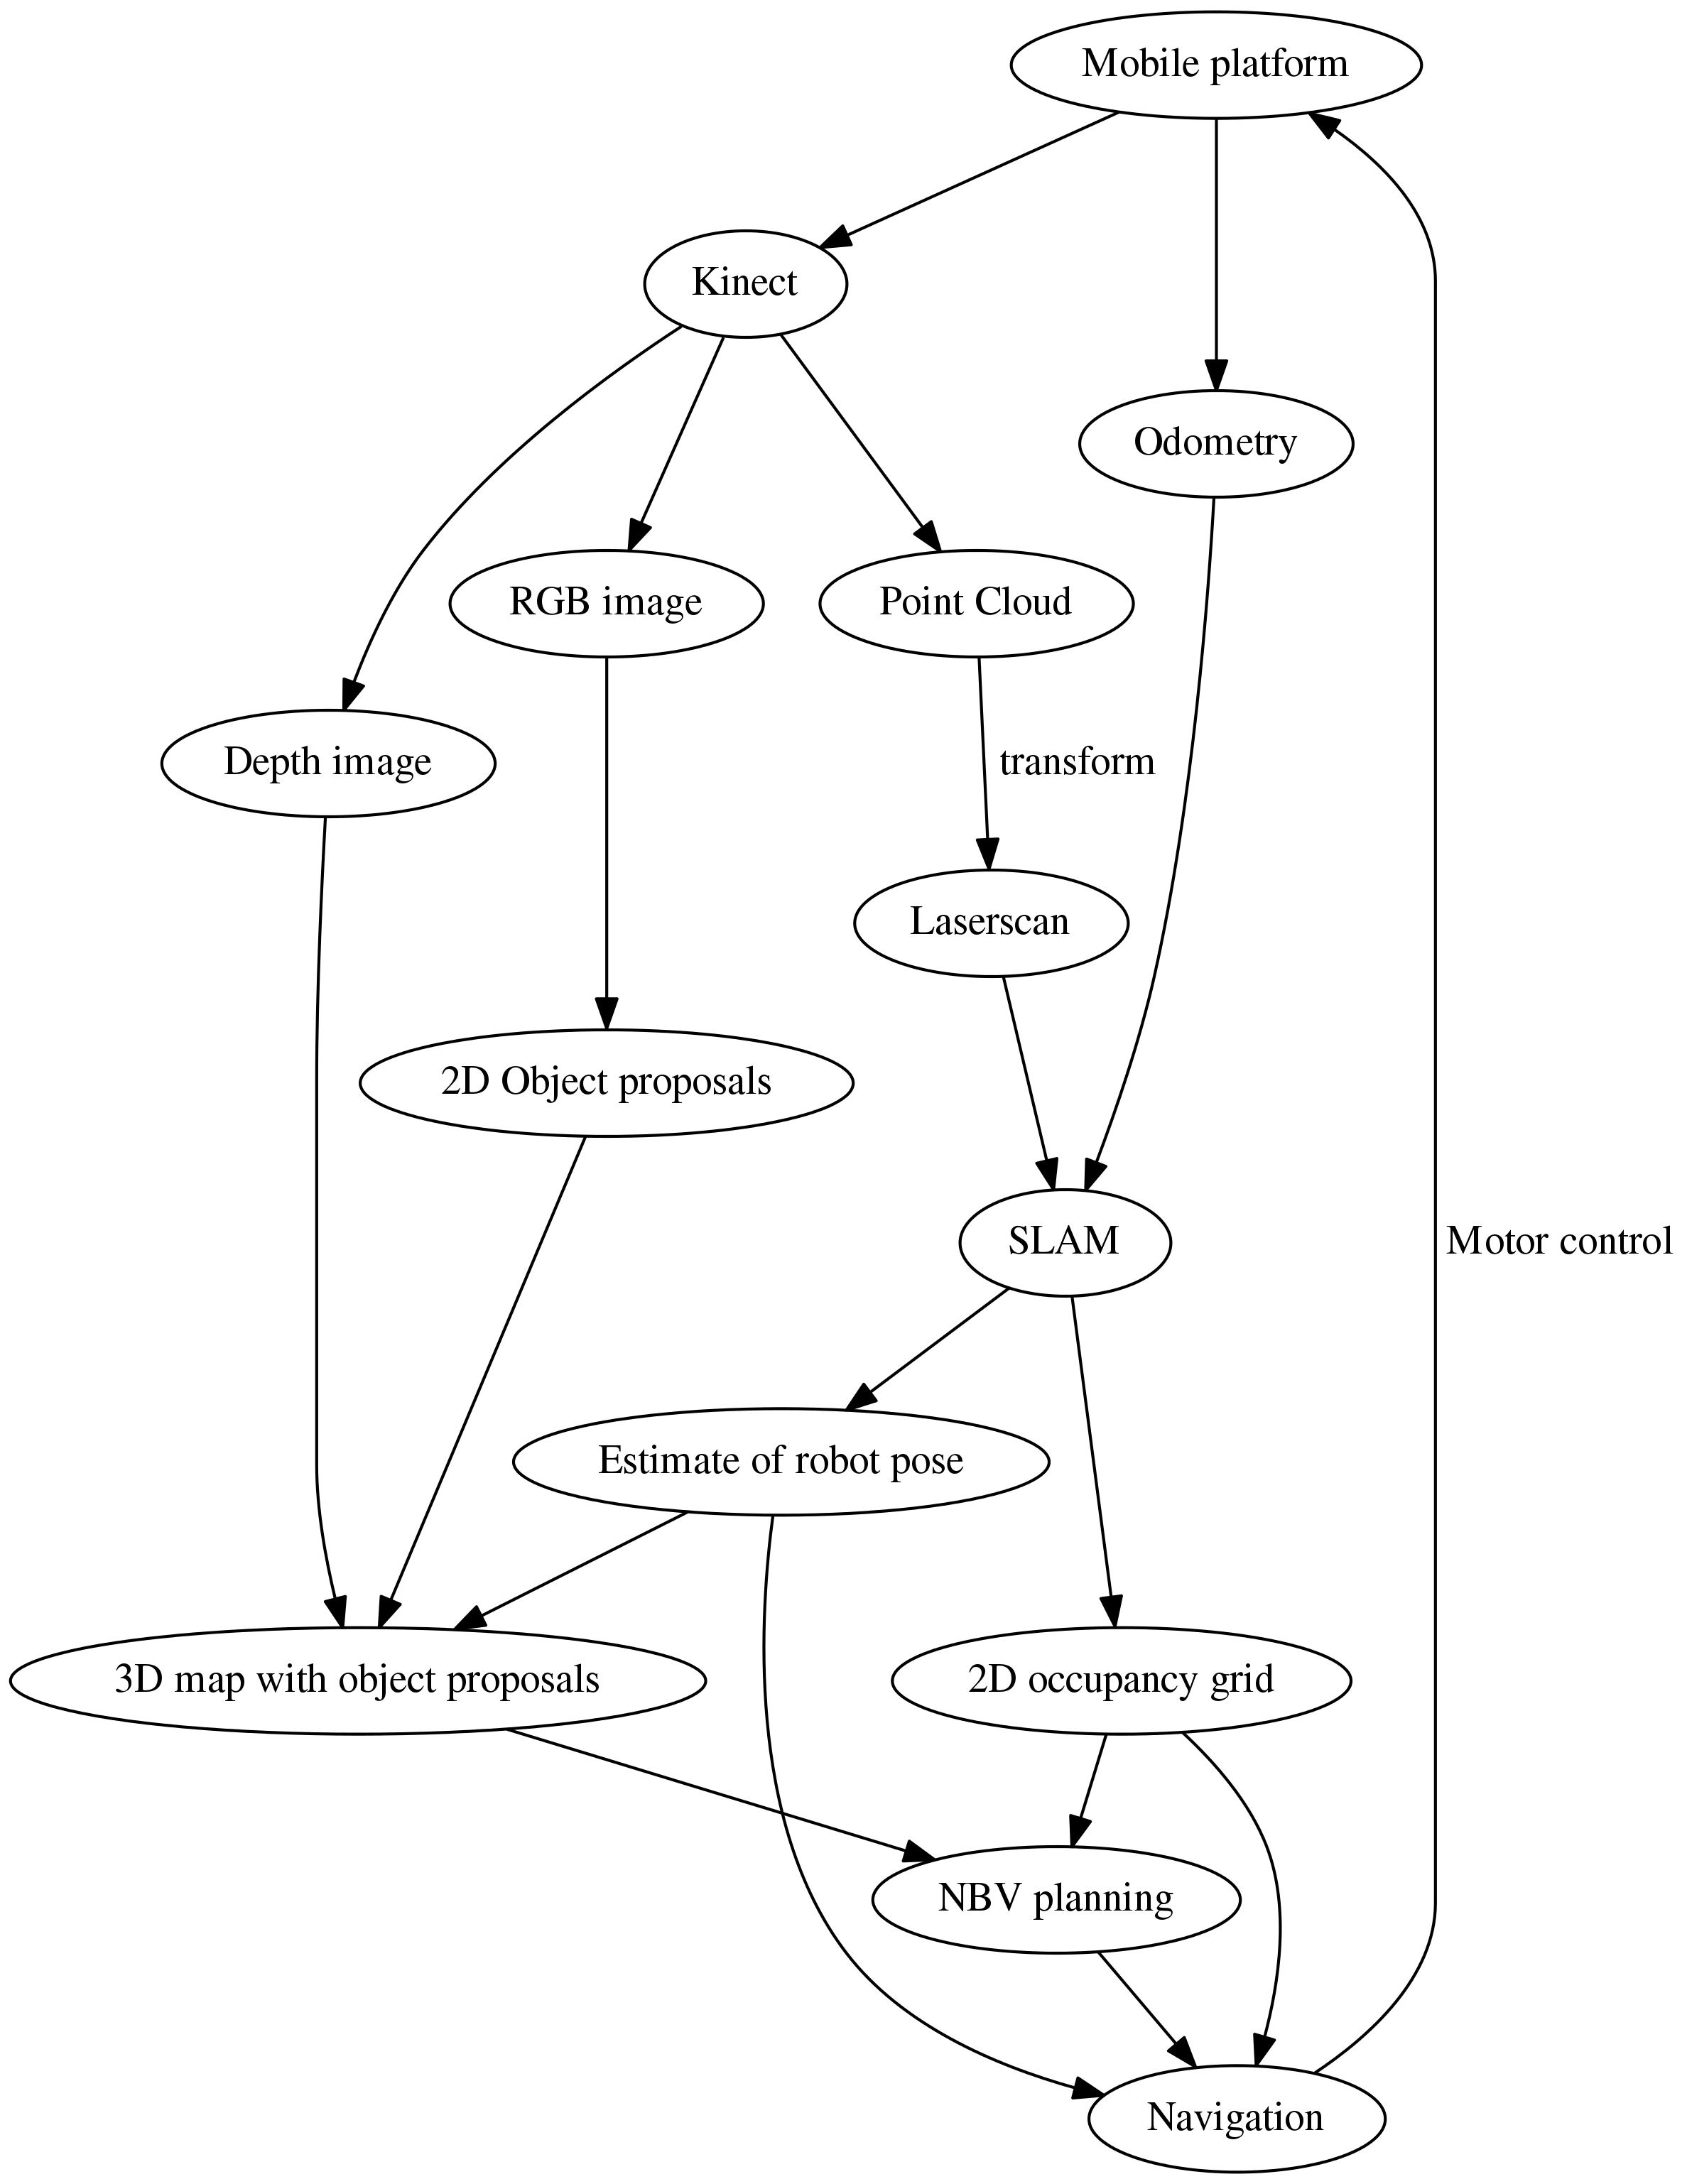
\includegraphics[width=0.82\linewidth]{dot/overview.png} 
		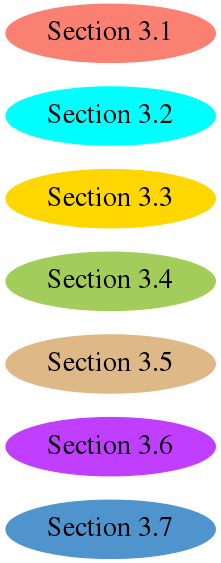
\includegraphics[width=0.17\linewidth]{dot/legend.png} 
		\caption{Overview of the information flow in the system}
		\label{fig:overview}
	\end{center}
\end{figure}

A general overview of the system is given in Figure \ref{fig:overview}.

The input consists of the odometry from the mobile platform and the depth image, colour image, and point cloud data from the mounted RGB-D camera.
Our SLAM algorithm requires laser scan data and the odometry, therefore we transform the point cloud to a simulated laser scan.
The SLAM algorithm provides us with an estimate of the robot's current pose and a 2D occupancy grid: a map of the environment in which each grid cell is set as containing either an obstacle, free space, or unexplored space. 

A new set of object proposals is computed in our system only at each NBV.
Between NBV poses, the camera data is used to improve the map, but not to find further objects.

Our object proposals are at first generated in 2D from the RGB image, then a corresponding point cloud for the object proposal is generated using the available depth information.
This point cloud is further processed to ensure that it represents a contiguous volume.
% To ensure that the object proposal point cloud corresponds to one contiguous volume a clustering algorithm is applied.
% Further processing is done only on the object proposal point cloud cluster closest to the robot. 
The cloud is then projected, with help of the estimated robot pose, into a 3D map, where the new object proposals are merged with already-existing ones.
% 3D object proposals that already have been integrated into the map previously are updated with the new proposals.

We try different NBV algorithms, which can work with the robot's current pose, the 2D map of the environment, and with knowledge about the approximated object positions.
As output of each NBV algorithm we receive the next desired robot pose.
This is then used together with the 2D map and the approximated robot position to navigate the robot.

% A more detailed description of the implementation of the different parts of our system is given in Section \ref{Implementation}.

% subsection system_overview (end)

\section{Theoretical background}
\label{Theoretical_background}
%Theoretical background, which provides the descriptions on what existing theories and ideas that are related to your problem statement. The purpose of this section is to ensure that you are knowledgeable about the related key concepts, theories and models. Do not copy your text from the intermediate report. Revise and rewrite according to the feedback you got and what the actual outcome of the project was.

In this section we present some of the concepts and methods that we utilize in our system.

\subsection{Saliency-based object discovery}
\label{Theoretical_background:Saliency-based_object_discovery}
To find objects in the robots current view, we use a saliency-based object discovery system.
Such a system has been introduced by García et al. \cite{garcia2015saliency}.
An overview of the method can be seen in Figure \ref{fig:2Dobject_discovery}.

\begin{figure}[h!]
	\begin{center}
		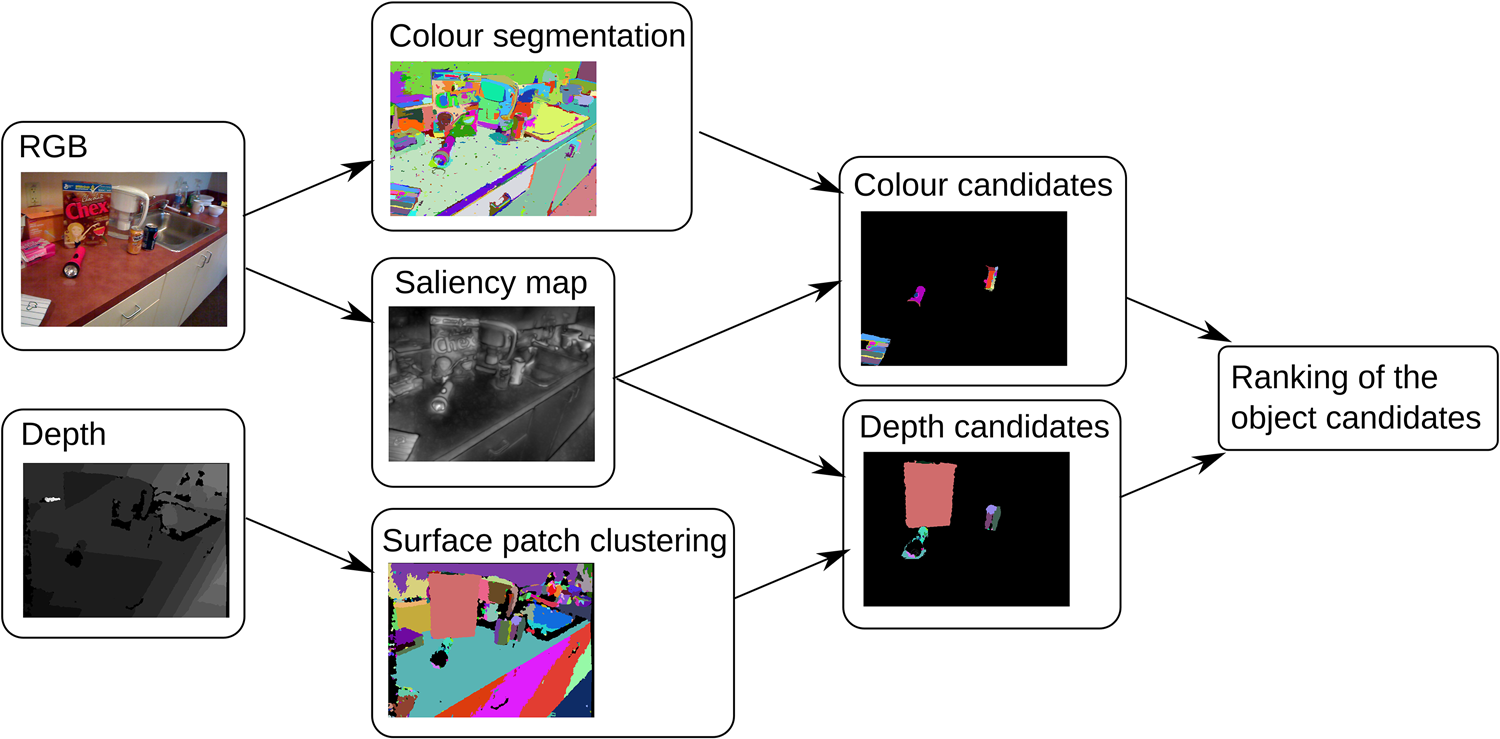
\includegraphics[width=1\textwidth]{src/saliency_object_detection.png}
		\caption{ Overview of the object candidate generation process \cite{garcia2015saliency}}
		\label{fig:2Dobject_discovery}
	\end{center}
\end{figure}

The method requires a colour and depth image of the same scene.
While it would work with colour information only experiments of the authors have shown that the combination of both achieves the best results.
The colour image is processed in two different ways: 
Using the Felzenszwalb and Huttenlocher algorithm \cite{felzenszwalb2004efficient} the image is segmented into small patches of similar colour.
Simultaneously a saliency map is computed. This is done with the VOCUS2 system developed by Frintrop et al. \cite{frintrop2015traditional}.
The general idea of VOCUS2 is to compute for each pixel a value quantifying its contrast to its proximate image area.
To generate object candidates the information of saliency map and colour segmentation are used together.
Seeded region growing is performed on the local maxima in the saliency map.
This means that starting from a local maxima neighboring pixels are iteratively grouped together into one region if their saliency value exceeds a certain percentage of the saliency value of the local maximum.
The result is a list of salient blobs in the saliency map.
For each salient blob one colour object candidate is created. It contains the pixels of all colour segments that overlap to at least $30\%$ with the pixels of the salient blob.
The depth candidates are generated analogous to the colour candidates, using the same salient blobs as a basis for the object candidates, but a surface clustering method is used as segmentation algorithm. It divides the image into continuous planes.
Afterwards, colour and depth candidates are merged into one set a ranking of proposed object candidates in terms of \glqq{}objectiveness\grqq{} takes place.

With more than 80\% recall and up to 50\% precision the saliency-based object discovery method performs comparable or better than other state-of-the-art object detection systems tested in the experiments of García et al.

\subsection{Frontier-based exploration}
\label{Theoretical_background:Frontier-based_exploration}
A method for autonomous exploration of unknown  environments has been introduced 1997 by Yamauchi \cite{yamauchi1997frontier}.
He describes the task that he wants to solve as follows: \glqq{}The central question in exploration is: \textit{Given what you know about the world, where should you move to gain as much  new  information  as  possible?}\grqq{}.
This is the same problem we have to solve for our object seeking robot.
Figure \ref{fig:frontier} presents how frontier-based exploration works.

\begin{figure}[h!]
	\begin{center}
		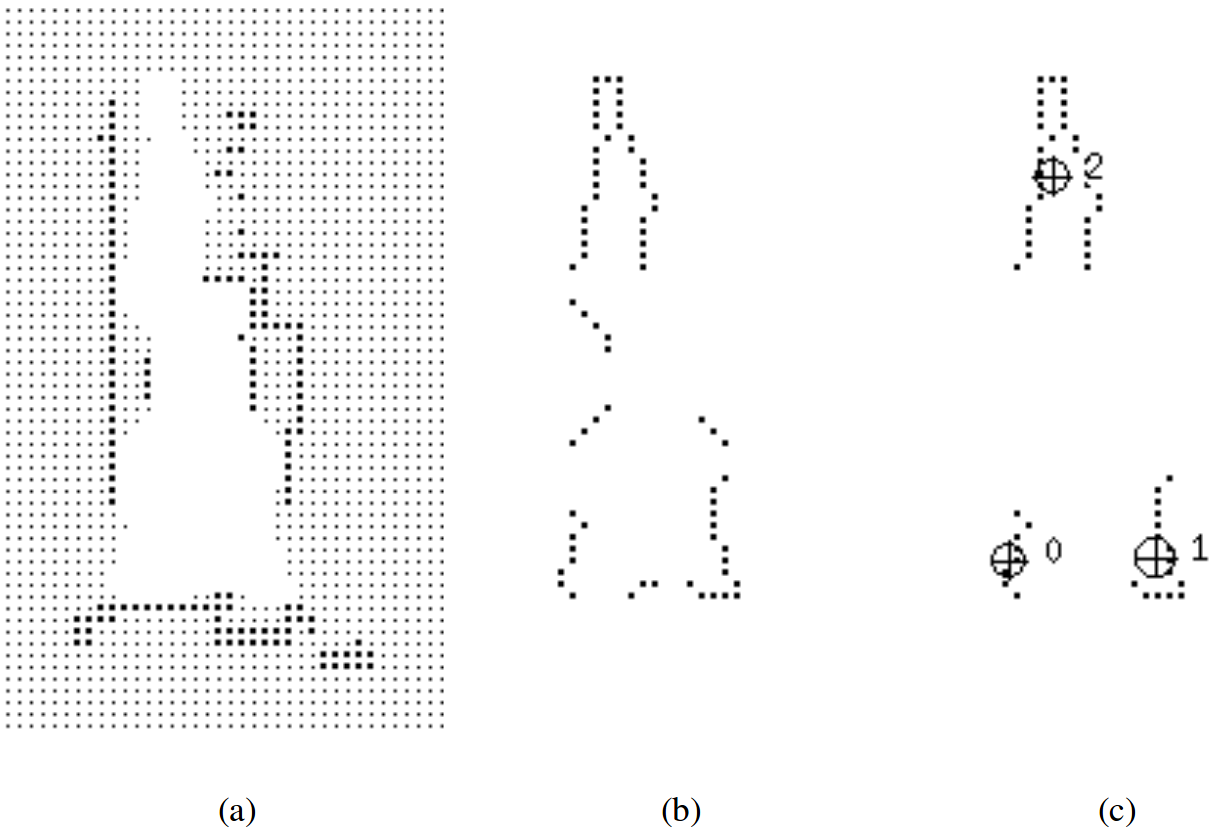
\includegraphics[width=.85\textwidth]{src/frontier_exploration.png}
		\caption{ Processing steps of frontier-based exploration \cite{yamauchi1997frontier}}
		\label{fig:frontier}
	\end{center}
\end{figure}

On the left (a) of the figure a possible map of the environment is depicted. Black dots represent unexplored cells of the map, stronger black dots mark found obstacles and white space is the available free space in which the robot should be able to navigate.
All cells on the border between free and unexplored space are marked in (b) as frontier edge segments.
Neighboring frontier edge segments are grouped together and if the contiguous space of the group is roughly larger than the robot, the group defines a frontier. The centroid of each frontier is represented by a crosshair in (c).
The robot will then navigate to the closest accessible frontier centroid and thereby explore the environment.

Yamauchi performed successful experiments using a Nomad 200 mobile robot in indoor environments.

\subsection{Sampling-based exploration}
\label{Theoretical_background:Sampling-based_exploration}
Sampling-based exploration is another way of finding a next best viewpoint to explore an initially unknown environment.
The general idea is to randomly sample the accessible area of the robot for possible viewpoints.
For each viewpoint a information gain score is computed, which depends on the visible area at the particular viewpoint and the distance of this viewpoint to the current robot position.

Such a system has been introduced by Surmann et al. \cite{surmann2003autonomous}.
For their system they use laser scanner data. From this data they detect obstacles, free space and unknown space.
The borders between free space and unknown space are called unseen lines.
Next best viewpoint candidates are randomly sampled from the free space.
For each of these candidates the number of visible unseen lines is computed, which determines its information gain.
The final score for each candidate is computed by multiplying the information gain with a punishing factor that depends on the euclidean distance to the current robot position and the angle that the robot would have to rotate for the view.
The next goal is then chosen as the viewpoint candidate with highest overall score.

%\subsection{Particle filter SLAM}
%\subsection{Euclidean point cloud clustering}
\subsection{IoR mechanism to guide attention}
\label{Theoretical_background:IoR mechanism_to_guide_attention}
An inhibition of return (IoR) mechanism can be used in computer vision to avoid spending attention on the same region for longer than necessary to process the information of that region.
Such a method is used in the object detection system by García et al. \cite{garcia2015saliency} to avoid the computation of the same object candidates in consecutive frames of a video sequence.
The system keeps track of previously considered object candidates through an 3D IoR map, which is a model of the environment built through a reconstruction algorithm (KinectFusion \cite{newcombe2011kinectfusion}) from the depth image of the RGB-D camera, where information about IoR is stored in the voxels of the map.
To update the IoR information in the map the current 2D camera frame is projected into the 3D map.
That way, voxels corresponding to the attended object candidates are found.
The IoR weight for each of these voxels is increased and if a certain threshold is reached an IoR flag is activated, signaling that pixels in the camera frame corresponding to this voxel should be inhibited.
For each frame that a voxel is not attended its IoR weight decreases and if it reaches zero again the IoR flag is deactivated.

The integration of this 3D IoR mechanism allowed García et al. to find most of the visible objects in a video while considering only a few object candidates per frame.

\subsection{Building a 3D map with octree data structure}
\label{Theoretical_background:Building_a_3Dmap_with_octree_data_structure}

%!TEX root = ../final_report.tex

While exploring the environment and discovering objects, the system needs to store a volumetric 3D representation of what it has discovered.
While this could be done by simply dividing the environment into a regular grid of voxels and storing information at each voxel, this is not an efficient way to store spatial information.
Often large subvolumes within the space are required to have the same information -- such as an object candidate label or a label for empty space -- at each of their constituent voxels, and explicitly representing and storing information at each voxel means the same information is stored many times.

One way of improving the efficiency of a volumetric representation is by using an octree\cite{meagher1982octrees}.
Octrees are an extension of the quadtree principle into 3D: at the top level sits a single root node, which represents the entire space to be mapped.
At the next level are eight nodes, each representing one eighth (octant) of the original cube.
This subdivision into eights recurses until the required level of granularity is reached (see figure \ref{fig:octree}).
Because each branch of the tree can be arbitrarily deep, information about a large volume of space can be stored once in a single high level tree node, rather than thousands of times in lowest-level voxels.
In areas where finer granularity is needed, the tree is deepened as required.
Thus the representation can be very fine-grained in areas where it needs to be, and much coarser-grained where such detail is not required.
% In theory an octree can be infinitely deep, although concrete implementations often place limits on the maximum tree depth.

\begin{figure}[ht]
	\begin{center}
		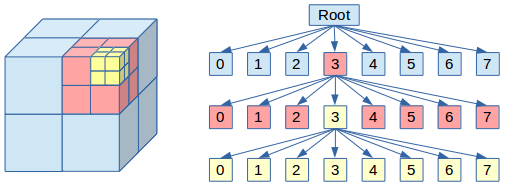
\includegraphics[width=0.6\linewidth]{src/octree.png} 
		\caption[Using an octree to represent a 3D volume]{Using an octree to represent a 3D volume.\footnotemark}
		\label{fig:octree}
	\end{center}
\end{figure}
\footnotetext{{\url{https://geidav.wordpress.com/2014/07/18/advanced-octrees-1- preliminaries-insertion-strategies-and-max-tree-depth}}}

\section{Implementation}
\label{Implementation}
%Implementation, which connects with the section on theoretical background and describes how the required parts were implemented, and how the overall system is constructed.

The general structure of our system has been introduced in Section \ref{Introduction} already.
We have mostly developed our system inside a physics simulation (Gazebo \footnote{\url{http://gazebosim.org/}}), however we transferred the system with slight adjustments onto a real Pioneer robot as well.
In the following we will explain how the different parts in Figure \ref{fig:overview} have been implemented. If the simulated and real version are diverging we will point that out in the respective system part description.
The system is fully developed with the Robot Operating System (ROS \footnote{\url{http://www.ros.org/}}) in the Indigo version, therefore each part of the system consists of one or multiple ROS nodes and services.
The code for our system can be found online \footnote{\url{https://github.com/Fabse92/cv_project}}.

\subsection{Mobile platform}
As mobile platform we used a Pioneer P3DX. This robot is providing a first estimate for its own position in form of odometry based on the previous motor control. Mounted onto the platform is a Kinect camera \footnote{\url{https://developer.microsoft.com/en-us/windows/kinect}}. In case of the real version we put the camera on top of the platform, in the physics simulation we are free of physical bounds and put the camera slightly lower in front of the robot to accommodate for our experimental setup in which objects are lying scattered on the floor.

\subsection{RGB-D camera}
The Kinect camera is directly providing a rectified version of the colour and depth image, which aligns the two frames, therefore pixel coordinates both images are corresponding to each other (\textbf{TODO is this correct?!}).
Also a point cloud build from the fused information of depth and colour image is directly provided as a ROS topic through the respective camera driver for simulation and real world.

\subsection{Laserscan}
To simulate a laser scanner we use the ros package \texttt{pointcloud\_to\_laserscan} \footnote{\url{http://wiki.ros.org/pointcloud_to_laserscan}}.
It receives the current point cloud from the RGB-D camera and samples the point cloud between a specified minimal and maximal height.
The closest point for each vertical line is put out to form one horizontal line which is our simulated laser scan.

\subsection{SLAM}
To perform simultaneous localization and mapping we use a ROS wrapper \footnote{\url{http://wiki.ros.org/gmapping}} for OpenSlam's GMapping algorithm \cite{grisetti2007}, which is an implementation of Fast SLAM.
GMapping performs laser-based SLAM using a particle filter.
It requires laser scan data and the estimated current robot position and provides a 2D occupancy grid map and the transform of the robot's pose into the map frame.
The occupancy grid map consists of cells of specified size.
Each cell can take one of four possible values.
The cell is thereby marked as obstacle, free space, unexplored space or as inscribed inflated obstacle, which means that this cell is not accessible by the robot since according to its footprint it would be in collision with an obstacle.

\subsection{Generation of object proposals}
The generation of object proposals is a complex part of the system that consists of five separate processing steps that we describe individually.

\subsubsection{2D Object candidate generation}
The first step in our method for object proposal generation is to find 2D object proposals in the current colour camera frame.
To achieve this we use the framework of García et al. presented in Section \ref{Theoretical_background:Saliency-based_object_discovery}.
We are currently only using the colour candidates. The object proposals contain usually most of the objects in the image and are of good quality, therefore we left the integration of the additional depth candidates for possible future work.
In Figure \ref{fig:object_generation} an example for the generation of object proposal is depicted.

\begin{figure}[h!]
	\begin{center}
		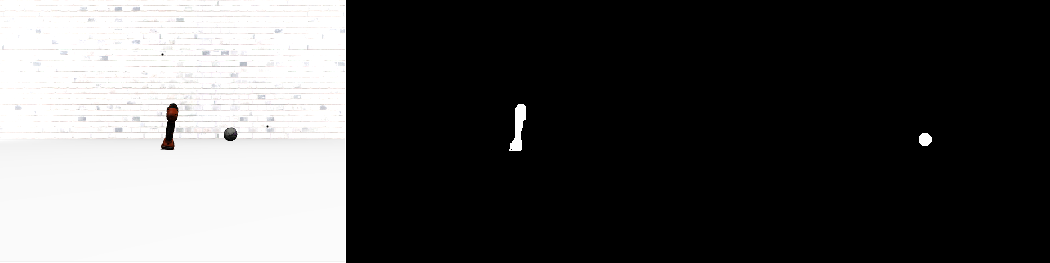
\includegraphics[width=1\textwidth]{src/object_generation.png}
		\caption{Left: Current camera image. Middle: First object proposal. Right: Second object proposal.}
		\label{fig:object_generation}
	\end{center}
\end{figure}

In our implementation of the framework of García et al. we start by computing a saliency map using VOCUS2 \cite{frintrop2015traditional}.
The colour segmentation is done using a C++ implementation of the Felzenszwalb and Huttenlocher algorithm \cite{felzenszwalb2004efficient} by Christoffer Holmstedt \footnote{\url{https://github.com/christofferholmstedt/opencv-wrapper-egbis}}.
Starting with the pixel with highest saliency, we perform seeded region growing where iteratively neighboring pixels are appended to the current salient region if their saliency value is at least 65\% of the value from the starting pixel.
In order to only keep actually interesting regions, a salient region is only kept for further processing if it has at least a mean saliency value of 130 (from a maximum of 255).
In order to prevent a large amount of strongly overlapping salient blobs, we do the following: For each considered saliency maximum the pixels from a seeded region growing, now using minimum similarity of 90\%, are then no longer considered as potential starting points for further salient regions.
Still some  of the salient regions will have large overlap, if the overlap is greater than 50\% only the one with higher saliency score is kept.
Where the saliency score is calculated as mean saliency times square root of the area of the corresponding region.
All of the remaining salient blobs will now correspond to one object proposal.
At this point the segments from the Felzenszwalb and Huttenlocher algorithm are used.
For each salient blob we find the corresponding segments that have least 30\% overlap.
The sum of these segments is the region of the object proposal for this particular salient blob.

\subsubsection{Building the proposal point cloud}
\label{sssec:building_proposal_point_cloud}

The 2D object proposals are next projected into 3D.
For each pixel which is part of the 2D proposal, we use the known geometry of the camera to project a ray from the Kinect's optical centre through the centre of the pixel and out into the world.
The value from the corresponding pixel in the Kinect's rectified depth map tells us how far along this ray the nearest surface is, thus giving us a point in 3D space which lies on the surface of our object candidate.

\subsubsection{Clustering of the proposal point cloud}
One problem with our approach of finding object proposals in the 2D image with subsequent projection into the third dimension using the available depth information is that imprecise or incorrect 2D object boundaries lead to distorted 3D object proposals.
For example it happens that larger parts of a wall far behind an object or parts of the floor are mistaken as part of the object.
One anomaly that occurred very often for us can be seen in Figure  \ref{fig:rays}.

\begin{figure}[h!]
	\begin{center}
		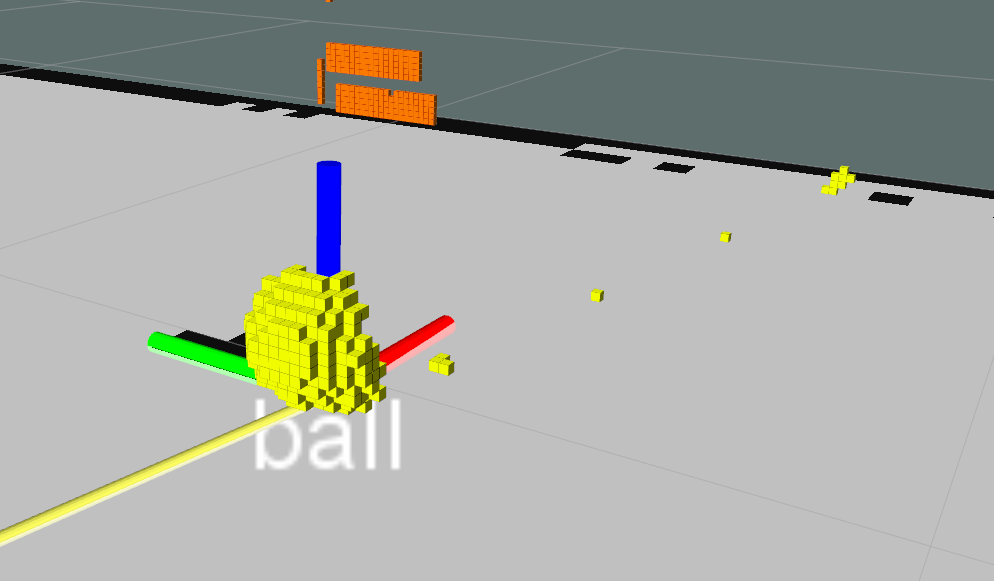
\includegraphics[width=0.5\textwidth]{src/rays2.png}
		\caption{Large parts of the ball are correctly identified; however, some additional voxels at the right side behind the ball are mistaken as belonging to the object.}
		\label{fig:rays}
	\end{center}
\end{figure}

To avoid this behavior we added an additional step. 
The obtained proposal point cloud is clustered using PCLs Euclidean Cluster Extraction method.
This is a simple clustering algorithm.
The user defines a distance threshold.
All points that are closer as the distance threshold will end up in the same cluster.
For the further processing we use only the cluster with the closest point to the camera that has at least 50 points.
This is removing some of the anomalies, because the wrong parts of the object proposal will mostly be behind the actual object.

%!TEX root = ../final_report.tex

% \subsubsection{Building the proposal point cloud}
% \label{sssec:building_proposal_point_cloud}

% The 2D object proposals are next projected into 3D.
% For each pixel which is part of the 2D proposal, we use the known geometry of the camera to project a ray from the Kinect's optical centre through the centre of the pixel and out into the world.
% The value from the corresponding pixel in the Kinect's rectified depth map tells us how far along this ray the nearest surface is, thus giving us a point in 3D space which lies on the surface of our object candidate.

% \subsubsection{Clustering the point cloud}

% An issue which we discovered during the implementation phase was that the projection just described in \ref{sssec:building_proposal_point_cloud} has a certain amount of error.
% Because of this error, the pixels on the outer edge of the 2D candidate would often be projected not onto the object surface but past it, meaning points on the wall or floor beyond the object would be included in the candidate point cloud (see figure\todo{FIGURE}). 

% We first attempted to overcome this difficulty by simply eroding the outermost ring of pixels from the 2D candidate before performing the projection.
% However, we found that this only reduced the problem rather than solving it completely, and eroding more than a single ring of pixels from the 2D candidate resulted in an unacceptable distortion of the candidate's shape\todo{Make this sentence better}.

% In our final system, we project the entire 2D candidate and then perform Euclidean clustering on the resulting point cloud to remove outliers.
% \todo{Fuller description}
% \todo{References}

\subsubsection{Integration of point cloud into map}

The next step in our pipeline is to convert the candidate point cloud into a volumetric representation and integrate it into our octree-based 3D map.
% The 3D mapping is handled by the ROS packages \textit{octomap_mapping}\footnote{\url{http://wiki.ros.org/octomap_mapping}} and \textit{octomap_server}\footnote{\url{http://wiki.ros.org/octomap_server}}.
The octree itself is managed by the OctoMap framework\cite{hornung13octomap}, with ROS integration provided by the ROS package \textit{octomap}\footnote{\url{http://wiki.ros.org/octomap}}.
Off the shelf, the \textit{octomap} package allows for the incremental creation of a 3D occupancy grid map from point cloud data; our system extends this package to store not just occupancy information but also object candidate labels and certainty information at each node.
% \todo{Does this need more detail?}

% \subsubsection{Merging and handling of candidates in octomap}

For each point in the point cloud, \textit{octomap} calculates into which voxel the point falls, giving a set of voxels occupied by the new candidate.
This set of voxels is then compared to the data in the octree to see whether we already believe there to be an object at that location or whether we currently believe that the space is free.
If at least 95\% of the voxels in the new candidate are currently believed to be free, then the candidate is simply inserted into the map: the octree is updated such that all voxels in the candidate set are assigned the label of the new candidate with a certainty of \num{1}.\todo{Need to make the labelling process and certainty concept clearer}
However, if more than 5\% of the voxels in the new candidate are already labelled in the octomap, then the system calculates which existing object candidate the new candidate has the greatest overlap with.\todo{Add that the 5\% threshold comes from Garcia et al?}
Each voxel in the new candidate set is then updated as follows:

\begin{itemize}
	\item If the voxel is currently unlabelled, it is assigned the label of the greatest overlap candidate and a certainty of \num{1}.
	\item If the voxel already has the label of the greatest overlap candidate, its certainty is increased by \num{1}.
	\item If the voxel has a different label to the greatest overlap label, its certainty is reduced by \num{1}. If this results in a certainty of zero, then it is assigned the greatest overlap label with a certainty of \num{1}.
\end{itemize}

% \subsubsection{Projection of point cloud into map}

% \subsubsection{Merging and handling of candidates in octomap}

\subsection{NBV planning}
In our current system five different next best view algorithms are available, which we will describe in their individual parts.
The goal of each of these algorithms is to find a next view point with high information gain.
All our methods use the occupancy grid map from GMapping for their computations.
A view consists of one cell of the map as goal position and a yaw orientation value.

\subsubsection{Random NBV}
Random NBV is the baseline method which we can use to assess the improvement through more sophisticated NBV methods.
For this method all currently accessible free space cells of the map are considered as next view position.
One of these cells is randomly selected and forms together with a random orientation the random NBV.

\subsubsection{Frontier-based exploration (\texttt{FBE})}
Our NBV method based on frontier exploration, which has been introduced in Section \ref{Theoretical_background:Frontier-based_exploration}, is performing frontier exploration as it has been implemented in the \texttt{frontier\_exploration} ROS package \footnote{\url{http://wiki.ros.org/frontier_exploration}}.
The next best view computed at a certain start position is here the centroid of the closest frontier with an orientation that corresponds to the continued line between the start position and the centroid of the closest frontier.
One essential flaw of this NBV method is that it works only until the environment has been completely discovered.

\subsubsection{Sampling-based exploration using obstacles (\texttt{SBE(Obs)})}
For this NBV method we use sampling-based exploration as described in Section \ref{Theoretical_background:Sampling-based_exploration}.
Here all accessible free space cells closer than $2$ meters and further than $20$ centimeters are considered as potential next best view position.
For each of these cells a random orientation is selected and all cells are found which are closer than $3$ meters and can be seen when the robot is looking in the selected orientation at this particular cell. This considers obstacles, therefore cells behind obstacles do not count as visible. %This is done by computing the part of a $3$ meter radius circle with center point corresponding to the selected orientation and an total angle that corresponds to the camera opening angle. Subsequently, for each pixel of the edge 
Each visible cell can contribute to the information gain at the potential viewpoint.
If a visible cell is part of the unexplored space or is an obstacle the information gain increases. Unexplored cells in front of an obstacle contribute an additional information gain bonus.
The idea is here that obstacles might correspond to objects and are therefore worth looking at.
Furthermore, unexplored space might contain undiscovered obstacles and objects, and an unexplored cell directly besides an obstacle has a high probability to be also part of this obstacle.
For each considered accessible free space cell we compute the sum of the information gain values of the visible cells considering the random orientation at the particular cell and multiply this value with a punishing factor depending on the distance of the cell to the current robot position.
Overall the information gain score $S$ is computed as:
\begin{align*}
 S &= (\mbox{sum of information gain})\cdot exp(-d\cdot \mbox{distance})
\end{align*}
Where $d$ is a constant that can be used to adjust how strongly distance is punished. We set $d$ to $0.05$ as it has been done in \cite{surmann2003autonomous}.
The NBV is then selected as the cell with corresponding chosen orientation that has the highest information gain score.

One problem that can occur for this NBV method is that the robot is moving close to a group of objects and the robot gets stuck continuously looking at this group of objects since they are close and looking at them is awarded with a lot of information gain score.
This is partly a desired behavior since multiple viewpoints on the same objects are necessary to increase the object proposal quality. However, if the robot gets stuck he will not find all objects distributed in the room.
To avoid getting stuck for too long, we implemented an inhibition of return (IoR) behavior. This concept has been introduced in Section \ref{Theoretical_background:IoR mechanism_to_guide_attention}.
We keep track of an IoR map that is similar to the occupancy grid map.
For each viewpoint taken, an the value in the IoR map for the obstacle cells the robot looked at is increased by $3$.
Obstacle cells that have not been looked at decrease their value in the IoR map by $1$.
For all future information gain scores obstacle cells with an IoR map value higher than $5$ provide no information gain.
Therefore, consecutive viewpoints taking a look at the same obstacle group have decreased information gain score, so that at some point the robot should move away from the group.

\subsubsection{Sampling-based exploration using obstacles and object candidates (\texttt{SBE(Obs+Cands)})}
This method is based on \texttt{SBE (obs)}.
The difference is that in addition to obstacles the current object candidates are considered as well for the information gain calculation.
Each visible cell at which currently an object is assumed to be will increase the information gain score and similar as before unexplored cells in front of object candidates will award an additional bonus information gain score.
The information gain $S_i$ for a cell $i$ with object candidate $j$ depends on the certainty $c_j$ into this candidate:
\begin{align*}
 S_i &= \mbox{inf\_object}\cdot 2^{-(c_j-1)}
\end{align*}
Where $\mbox{inf\_object}$ is the base value for object information gain. An object candidate with certainty $1$ will for example be awarded with $\mbox{inf\_object}$ information gain, a cell with candidate of certainty $2$, however, will only be awarded $\mbox{inf\_object}/2$.
The idea is here that object candidates with low certainty are worth more to look at, to increase the certainty.

\subsubsection{Combination of frontier and sampling-based exploration (\texttt{FBE plus})}
This method combines \texttt{FBE} and \texttt{SBE(obs)}.
Until the whole room is explored the frontier exploration method is used after that the sampling-based exploration takes over. 
The goal of this method is to overcome the limitation of frontier exploration, but exploit the positive behavior of frontier exploration to find a good sequence of views which allow to look at least once at all areas of the environment.

\subsection{Navigation}
For navigation we use the \texttt{move\_base} ROS package \footnote{\url{http://wiki.ros.org/move_base}}.
It requires the current robot position approximation, sensor transforms and sensor data and provides appropriate velocity commands to navigate the platform once a valid goal pose has been requested.

\section{Analysis}
\label{Analysis}
% Results, which contain the descriptions of the experiments conducted and presents their results.
In this section we describe the our experiments we conducted for the analysis of our system.
After explaining the experimental setups, we define the metrics we are measuring during system execution, introduce the experimental parameters and finally the results from our different experimental setups are presented.

\subsection{Experimental setups}
The experiments are done completely inside the simulation.
We built two different rooms which are used as environments, they can be seen in Figure \ref{fig:rooms}.

\begin{figure}[h!]
	\begin{center}
		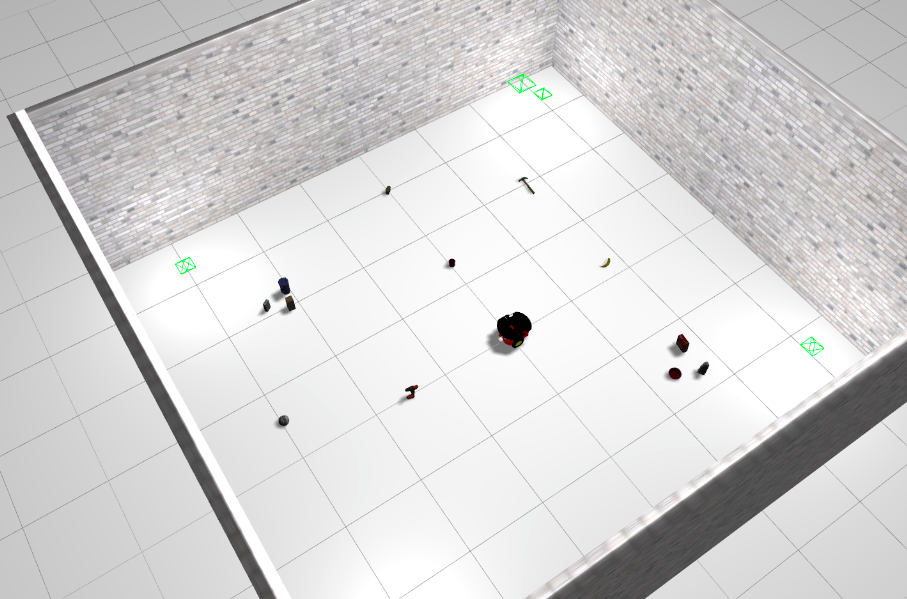
\includegraphics[width=0.49\textwidth]{src/clustered.png}
		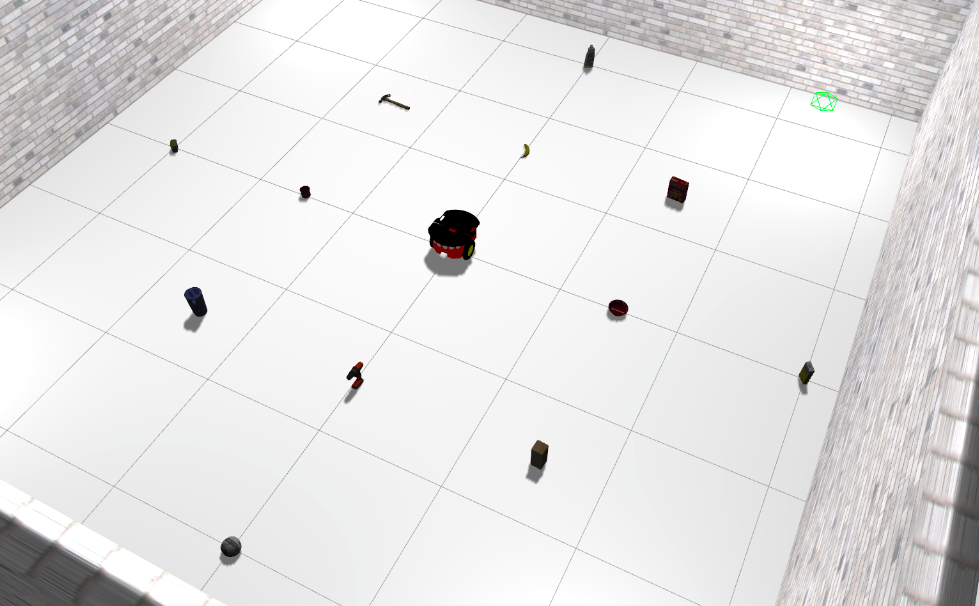
\includegraphics[width=0.49\textwidth]{src/scattered.png}
		\caption{Our two tested environments. The left one will be called \textit{clustered objects} and the right one \textit{scattered objects}}
		\label{fig:rooms}
	\end{center}
\end{figure}

In both rooms are $12$ of the larger objects from the YCB object and model set \cite{calli2015benchmarking}.
On the left is an environment which contains two groups of three objects which are close to each other and therefore has also some larger areas without any object.
On the right is an alternative room with equally distributed objects. The distance between the objects is here always $1.5$ meters. Both rooms have a size of roughly $7$ by $7$ meters.
In each of our experiments the robot is spawned in the middle of the room and we define the area which is allowed to be used for view positions. This area is slightly smaller than the room, which means that the walls are not included.
For the frontier exploration method this area also defines what has to be explored.
For the sampling based methods information gain is only provided for cells inside the boundaries.

During our first experimental test runs, we noticed that the approximated position through GMapping are strongly diverging from the actual robot position.
This leads to a lot of problems. It means that the map will become imprecise, the navigation becomes difficult and the projection of object candidates into the map frame is strongly diverging from the actual object position.
The diverging object proposal projection is the largest problem for our system and prevents us from receiving reasonable results. Therefore, we are running our experiments in default using a \textit{cheat mode}.
In this mode the actual camera position is provided for the object proposal projection into the map frame, the other parts of the system still have to work with the approximated position.

\subsection{Metrics}
The evaluation of object proposals happens after each view taken by the robot.

One of the simplest things to measure is the expired time since the beginning of the experiment.
For our time measurement we are subtracting the time used for the evaluation.

To evaluate the object proposals we use the metrics recall and precision on an object level.
Recall measures the percentage of available objects found by the system and precision measures the percentage of object proposals that where correct.
To determine if an object has been correctly found, we determine the object proposal with the largest overlap to it and compute the intersection over union (IoU) between the ground truth object and the proposal.
If the IoU is above some threshold the proposal is considered as correct.
The overlap between proposal and ground truth is computed by counting the voxels in the octomap which are occupied by both and from the sum of the overlapping voxels we can compute the overlapping volume.

\subsection{Further experimental parameters}
Besides which of the two environment to use and activated or deactivated cheat mode there are a couple of more parameters to select or vary for the experiments:

\begin{itemize}
	\item \textbf{Available time:} The time until the experiment is aborted. This is set to 25 minutes for our experiments.
	\item \textbf{IoU threshold:} Determines the IoU value necessary for an proposal to be considered correct. The threshold is set to $0.1$ for our experiments.
	\item \textbf{Information gain parameters:} For the sampling-based exploration methods up to five values determining the information gain per cell have to be set. The default values are: 2 for unexplored cells, 10 for cells containing obstacles, 20 for unexplored cells in front of obstacles, 100 for objects (multiplied with the factor depending on the proposal certainty) and 30 for unexplored cells in front of objects.
	\item \textbf{Minimal required proposal certainty:} The minimal proposal certainty necessary for an proposal to be considered for the evaluation. All proposals with lower certainty will be ignored. This parameter is per default set to $1$.
\end{itemize}

\subsection{Results}
In the following we present the results from our experiments.
Each experiment setting was run 25 times.
However, the system is crashing regularly. Most often because the robot thinks he is not able to move anymore.
In particular the \texttt{random NBV} method leads to many situations in which the robot can not move. Therefore, the \texttt{random NBV} method reached at most 13 views, while others were able to take up to 25 view poses.

At first we shall take a look at the development of recall and precision over the number of views taken.
This is depicted in Figure \ref{fig:recall_vs_nbv_count} and \ref{fig:precision_vs_nbv_count}.
Here we take the results from our room with scattered objects. Recall and precision curves are of similar shape but with slightly lower values overall for the room with some clustered objects.

\begin{figure}[h!]
	\begin{center}
		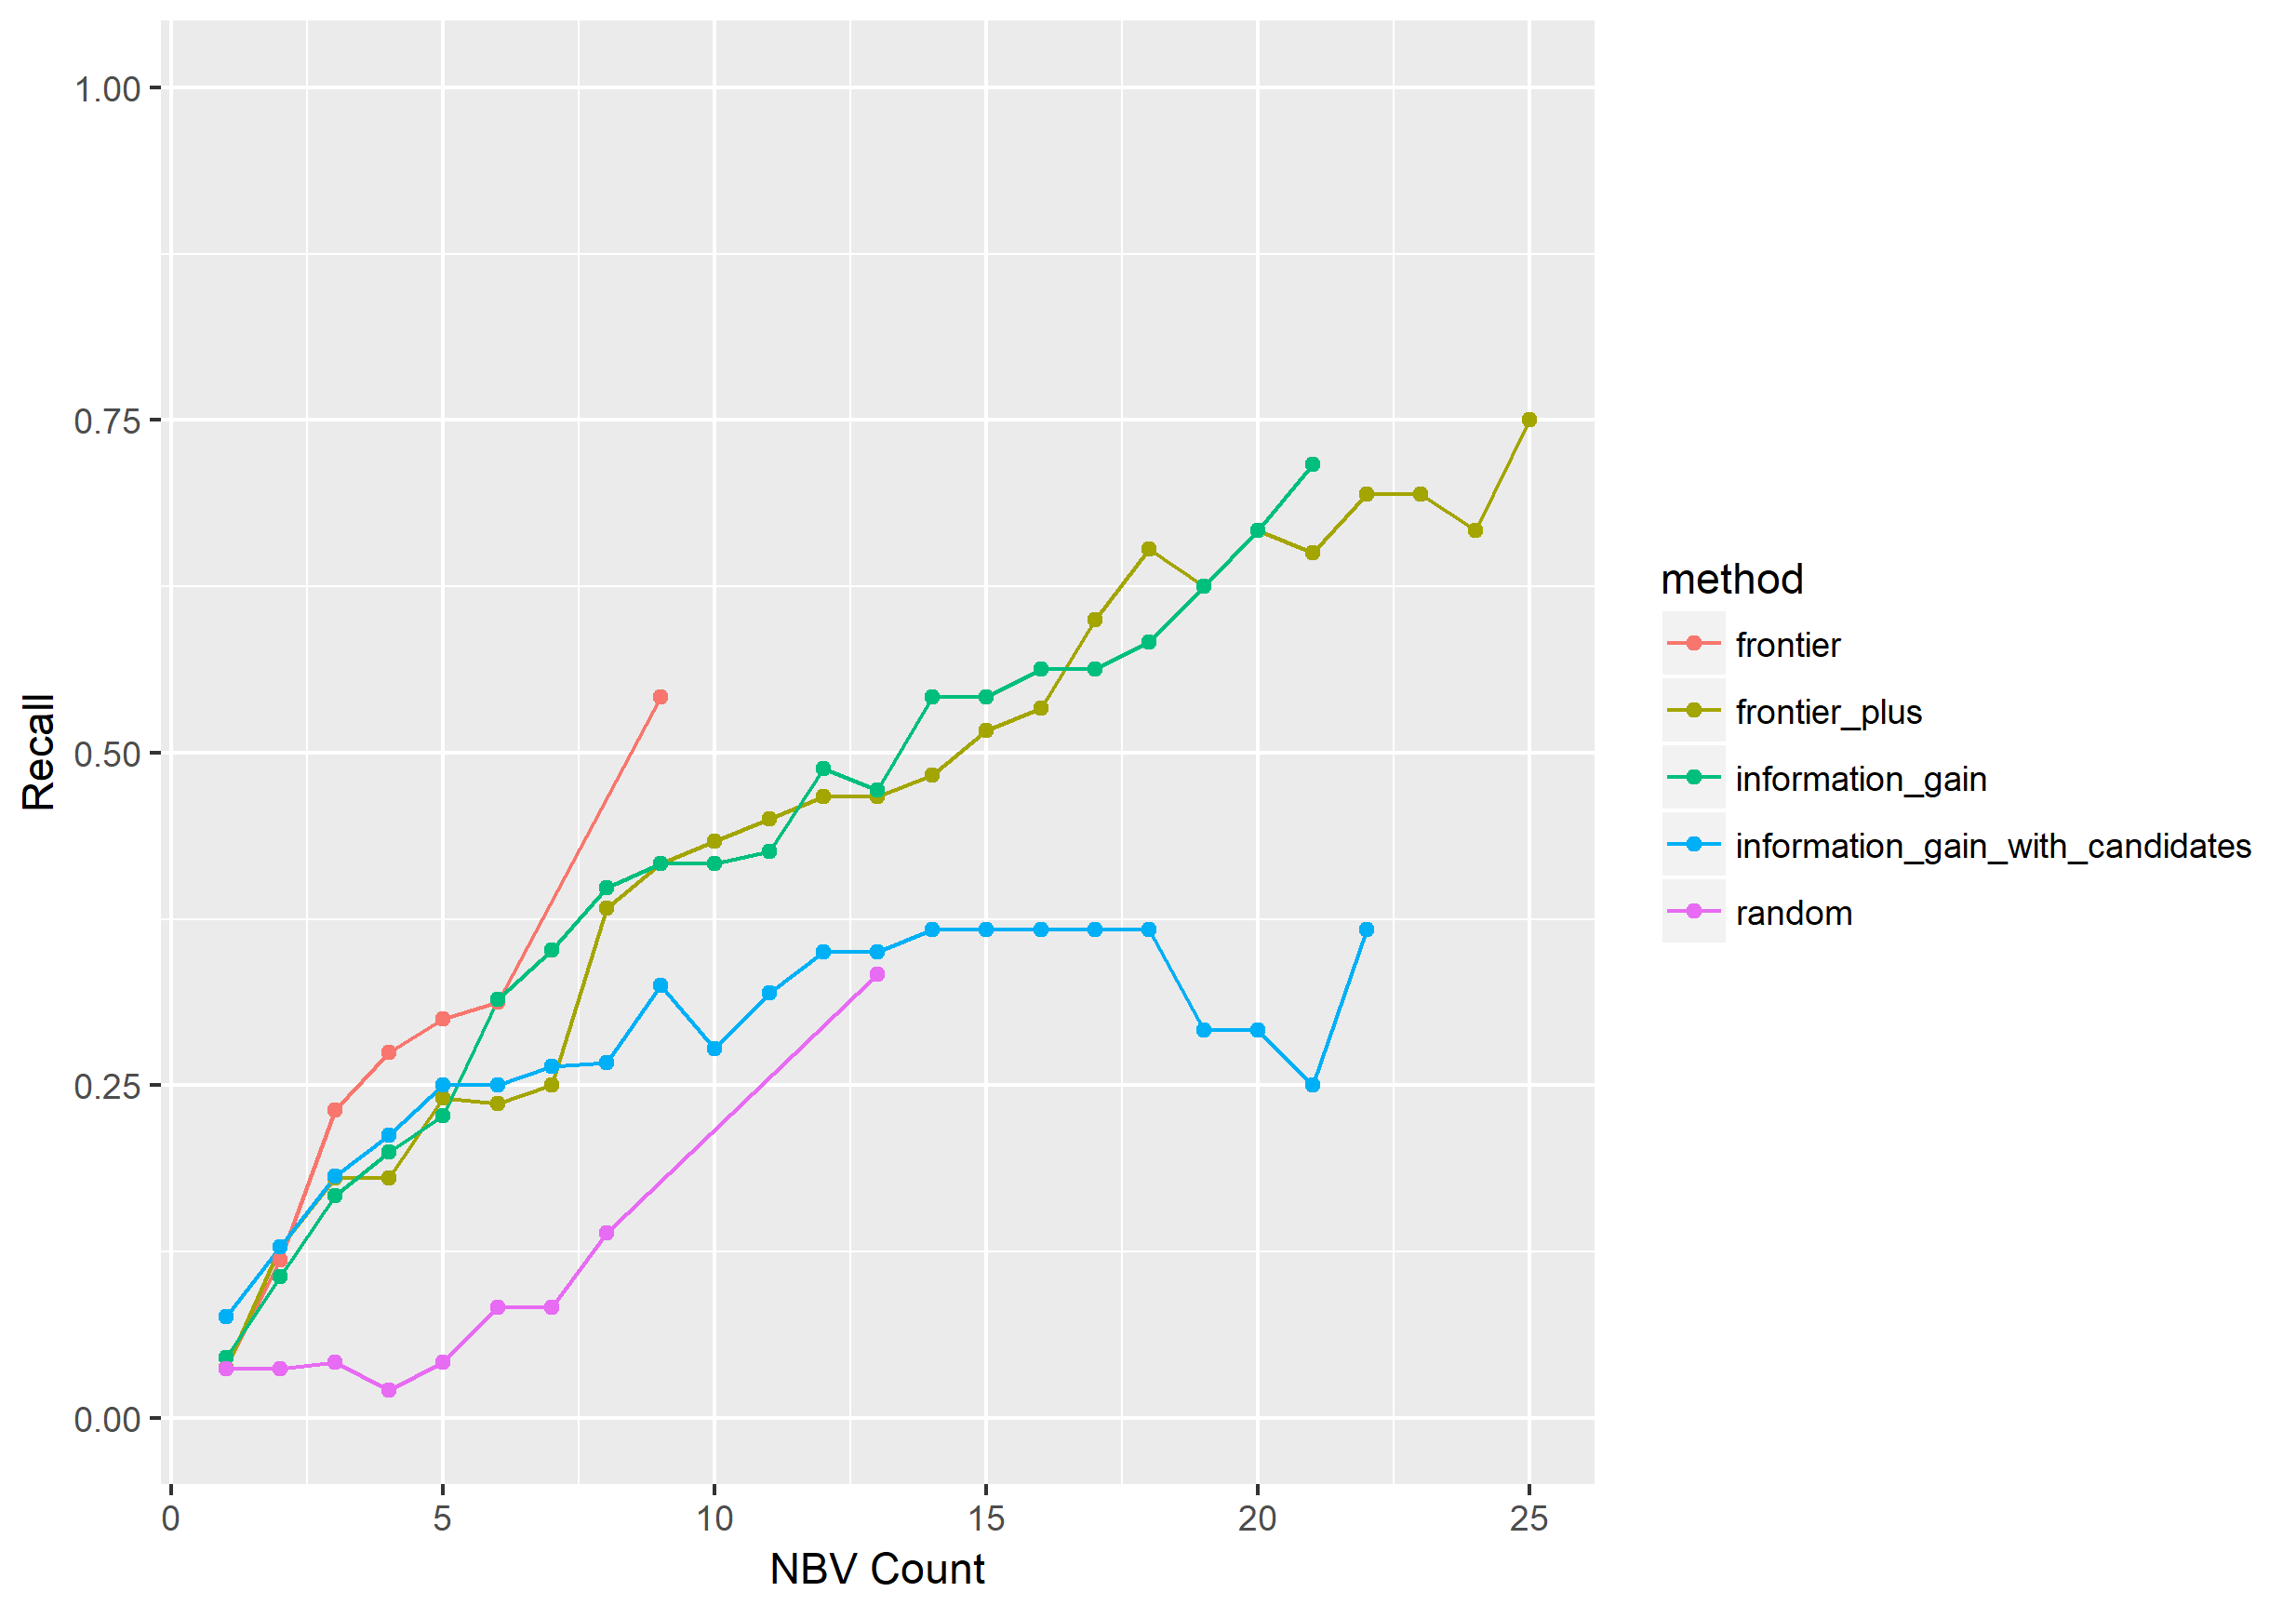
\includegraphics[width=1\textwidth]{src/Plots/recall_vs_nbv_count_scattered.png}
		\caption{Development of recall for all our NBV methods}
		\label{fig:recall_vs_nbv_count}
	\end{center}
\end{figure}

\begin{figure}[h!]
	\begin{center}
		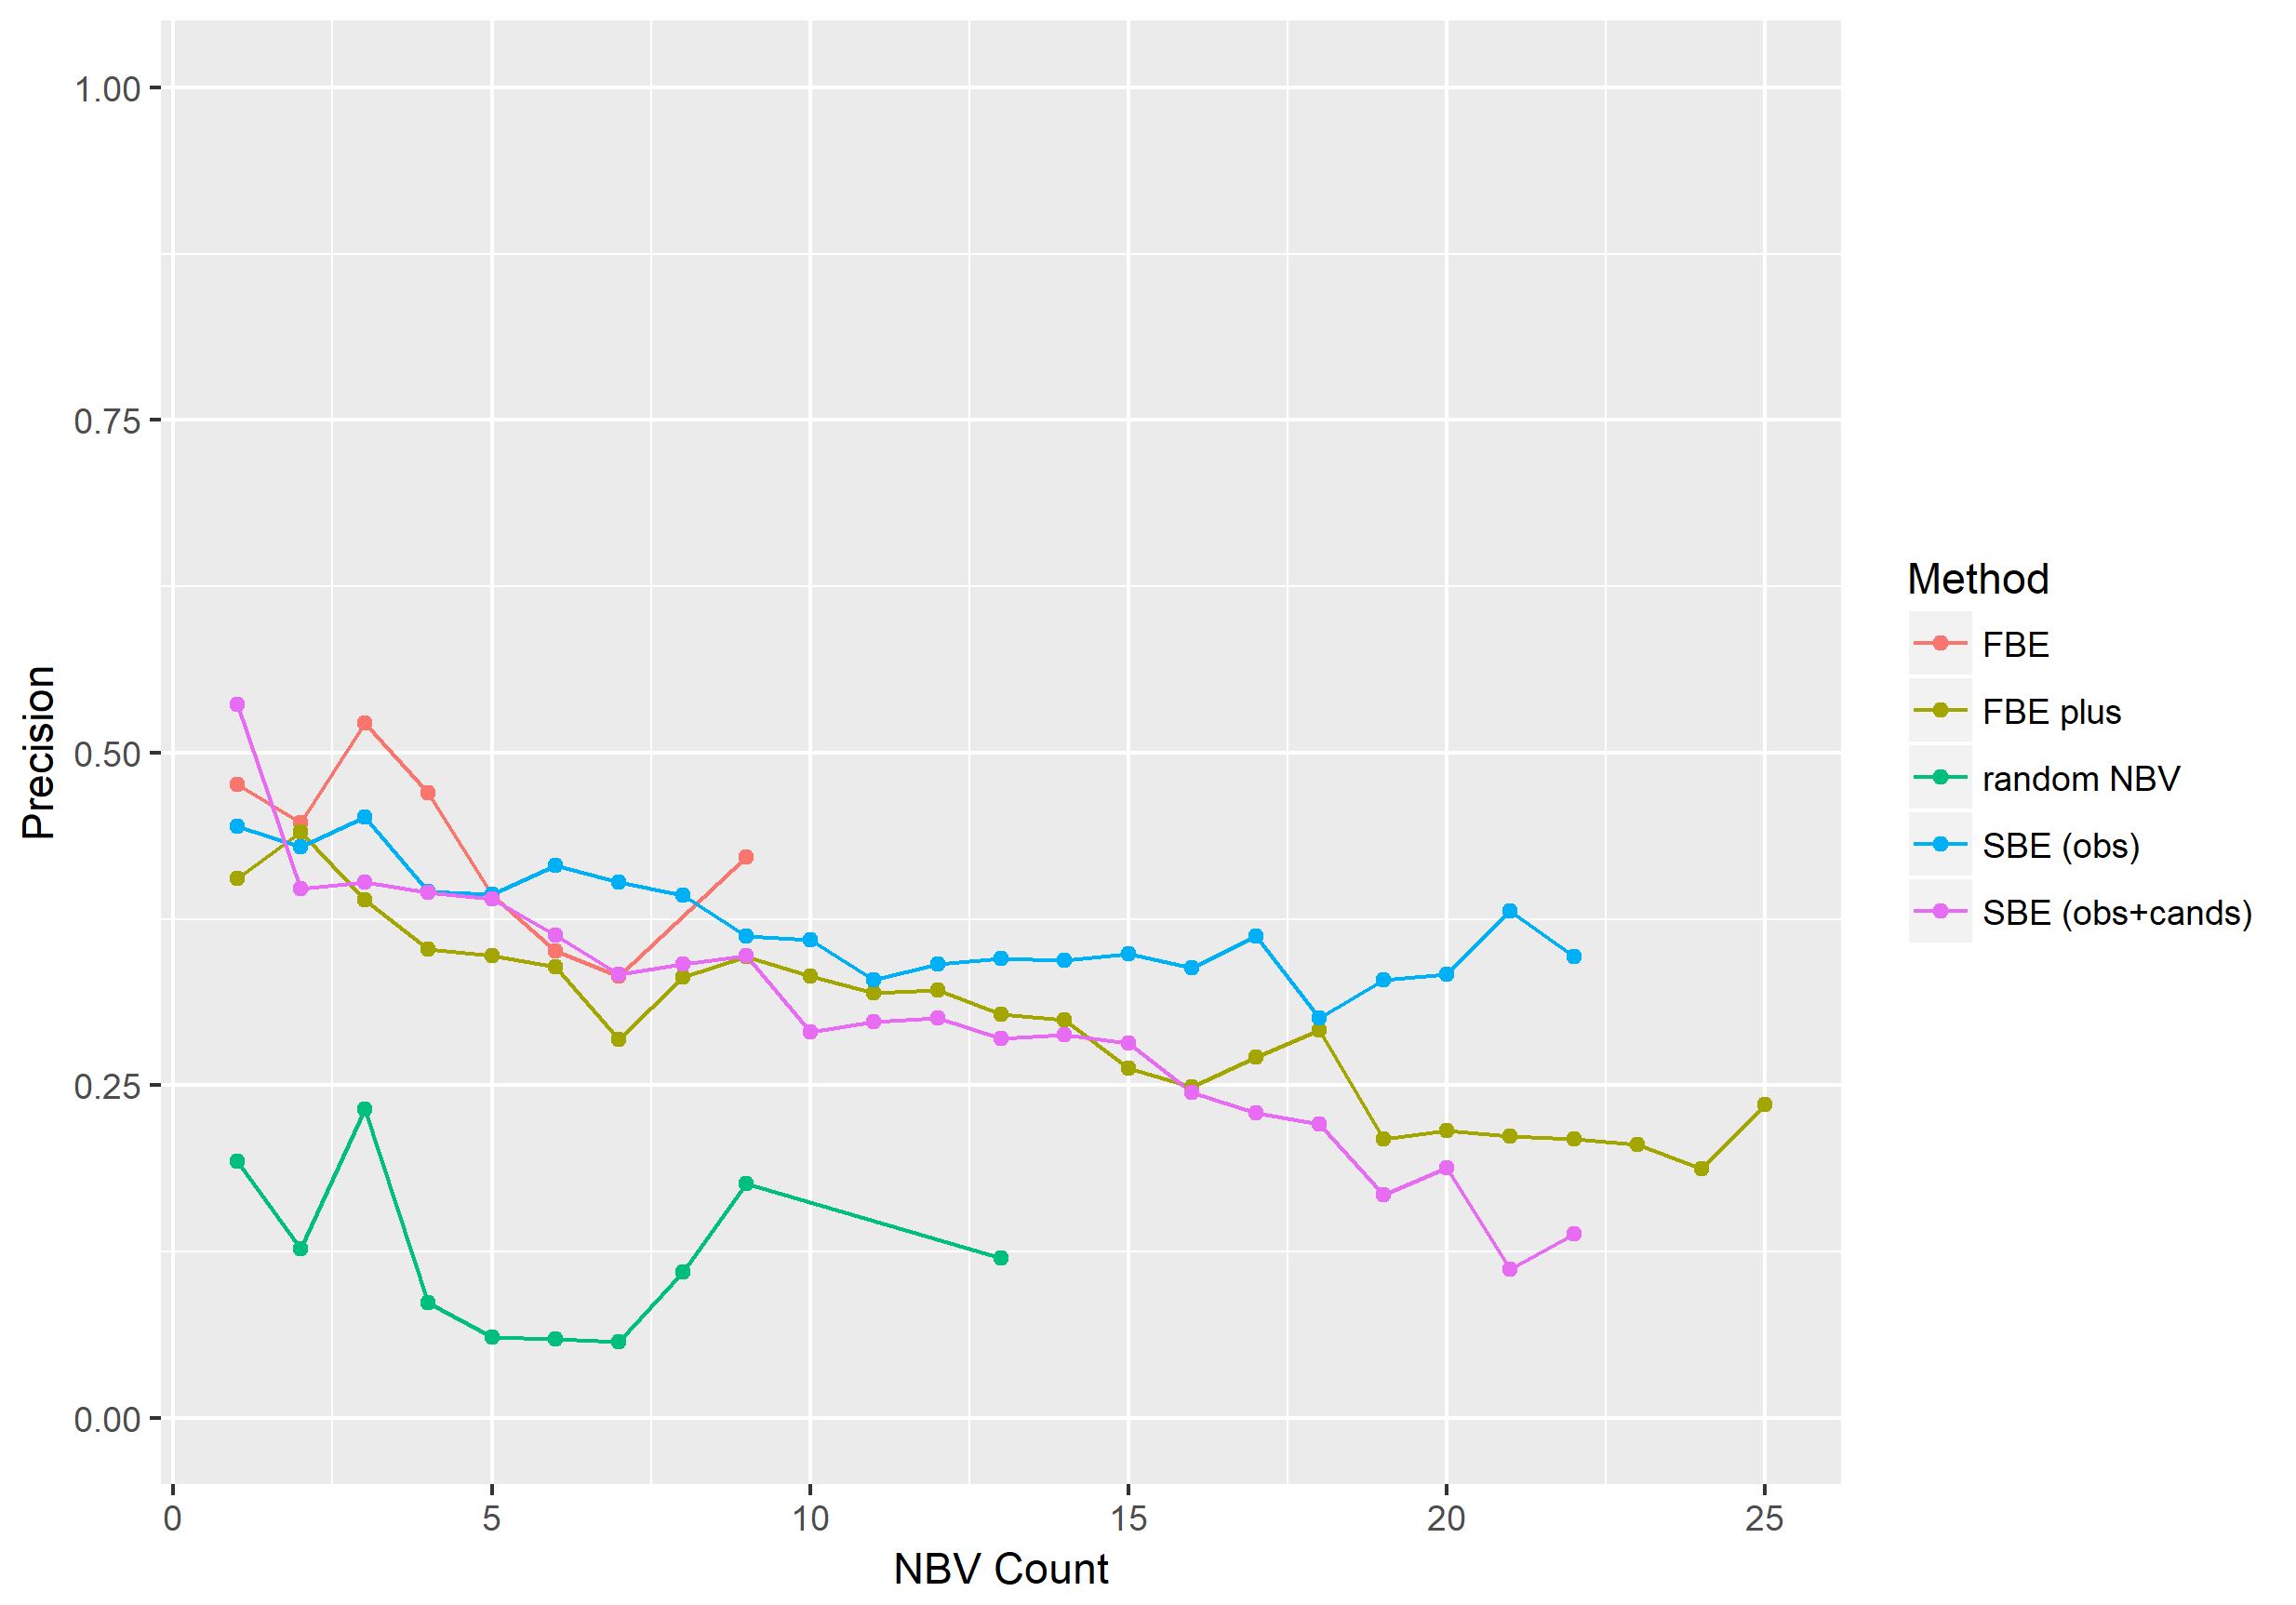
\includegraphics[width=1\textwidth]{src/Plots/precision_vs_nbv_count_scattered.png}
		\caption{Development of precision for all our NBV methods}
		\label{fig:precision_vs_nbv_count}
	\end{center}
\end{figure}

The best performing methods are \texttt{SBE(Obs)} and \texttt{FBE plus} which has the highest values for recall and precision.
They can reach recall values up to $0.75$ and have precision values between $0.25$ and $0.38$.
From the two graphs it becomes clear that all of the methods which somehow incorporate an information gain measure are more successful than the baseline method \texttt{random NBV}.
The \texttt{SBE(Obs+Cands)} is performing worse than than \texttt{SBE(Obs)}, our current assumption is that this is, because only about a quarter of objects are correct, thereby the robot gets more distracted from false object assumptions as he gets drawn to correct ones.
Variations between \texttt{FBE} and \texttt{FBE plus} and the beginning and between \texttt{FBE plus} and \texttt{SBE(Obs)} later occur through random fluctuations during the experiments.

\begin{figure}[h!]
	\begin{center}
		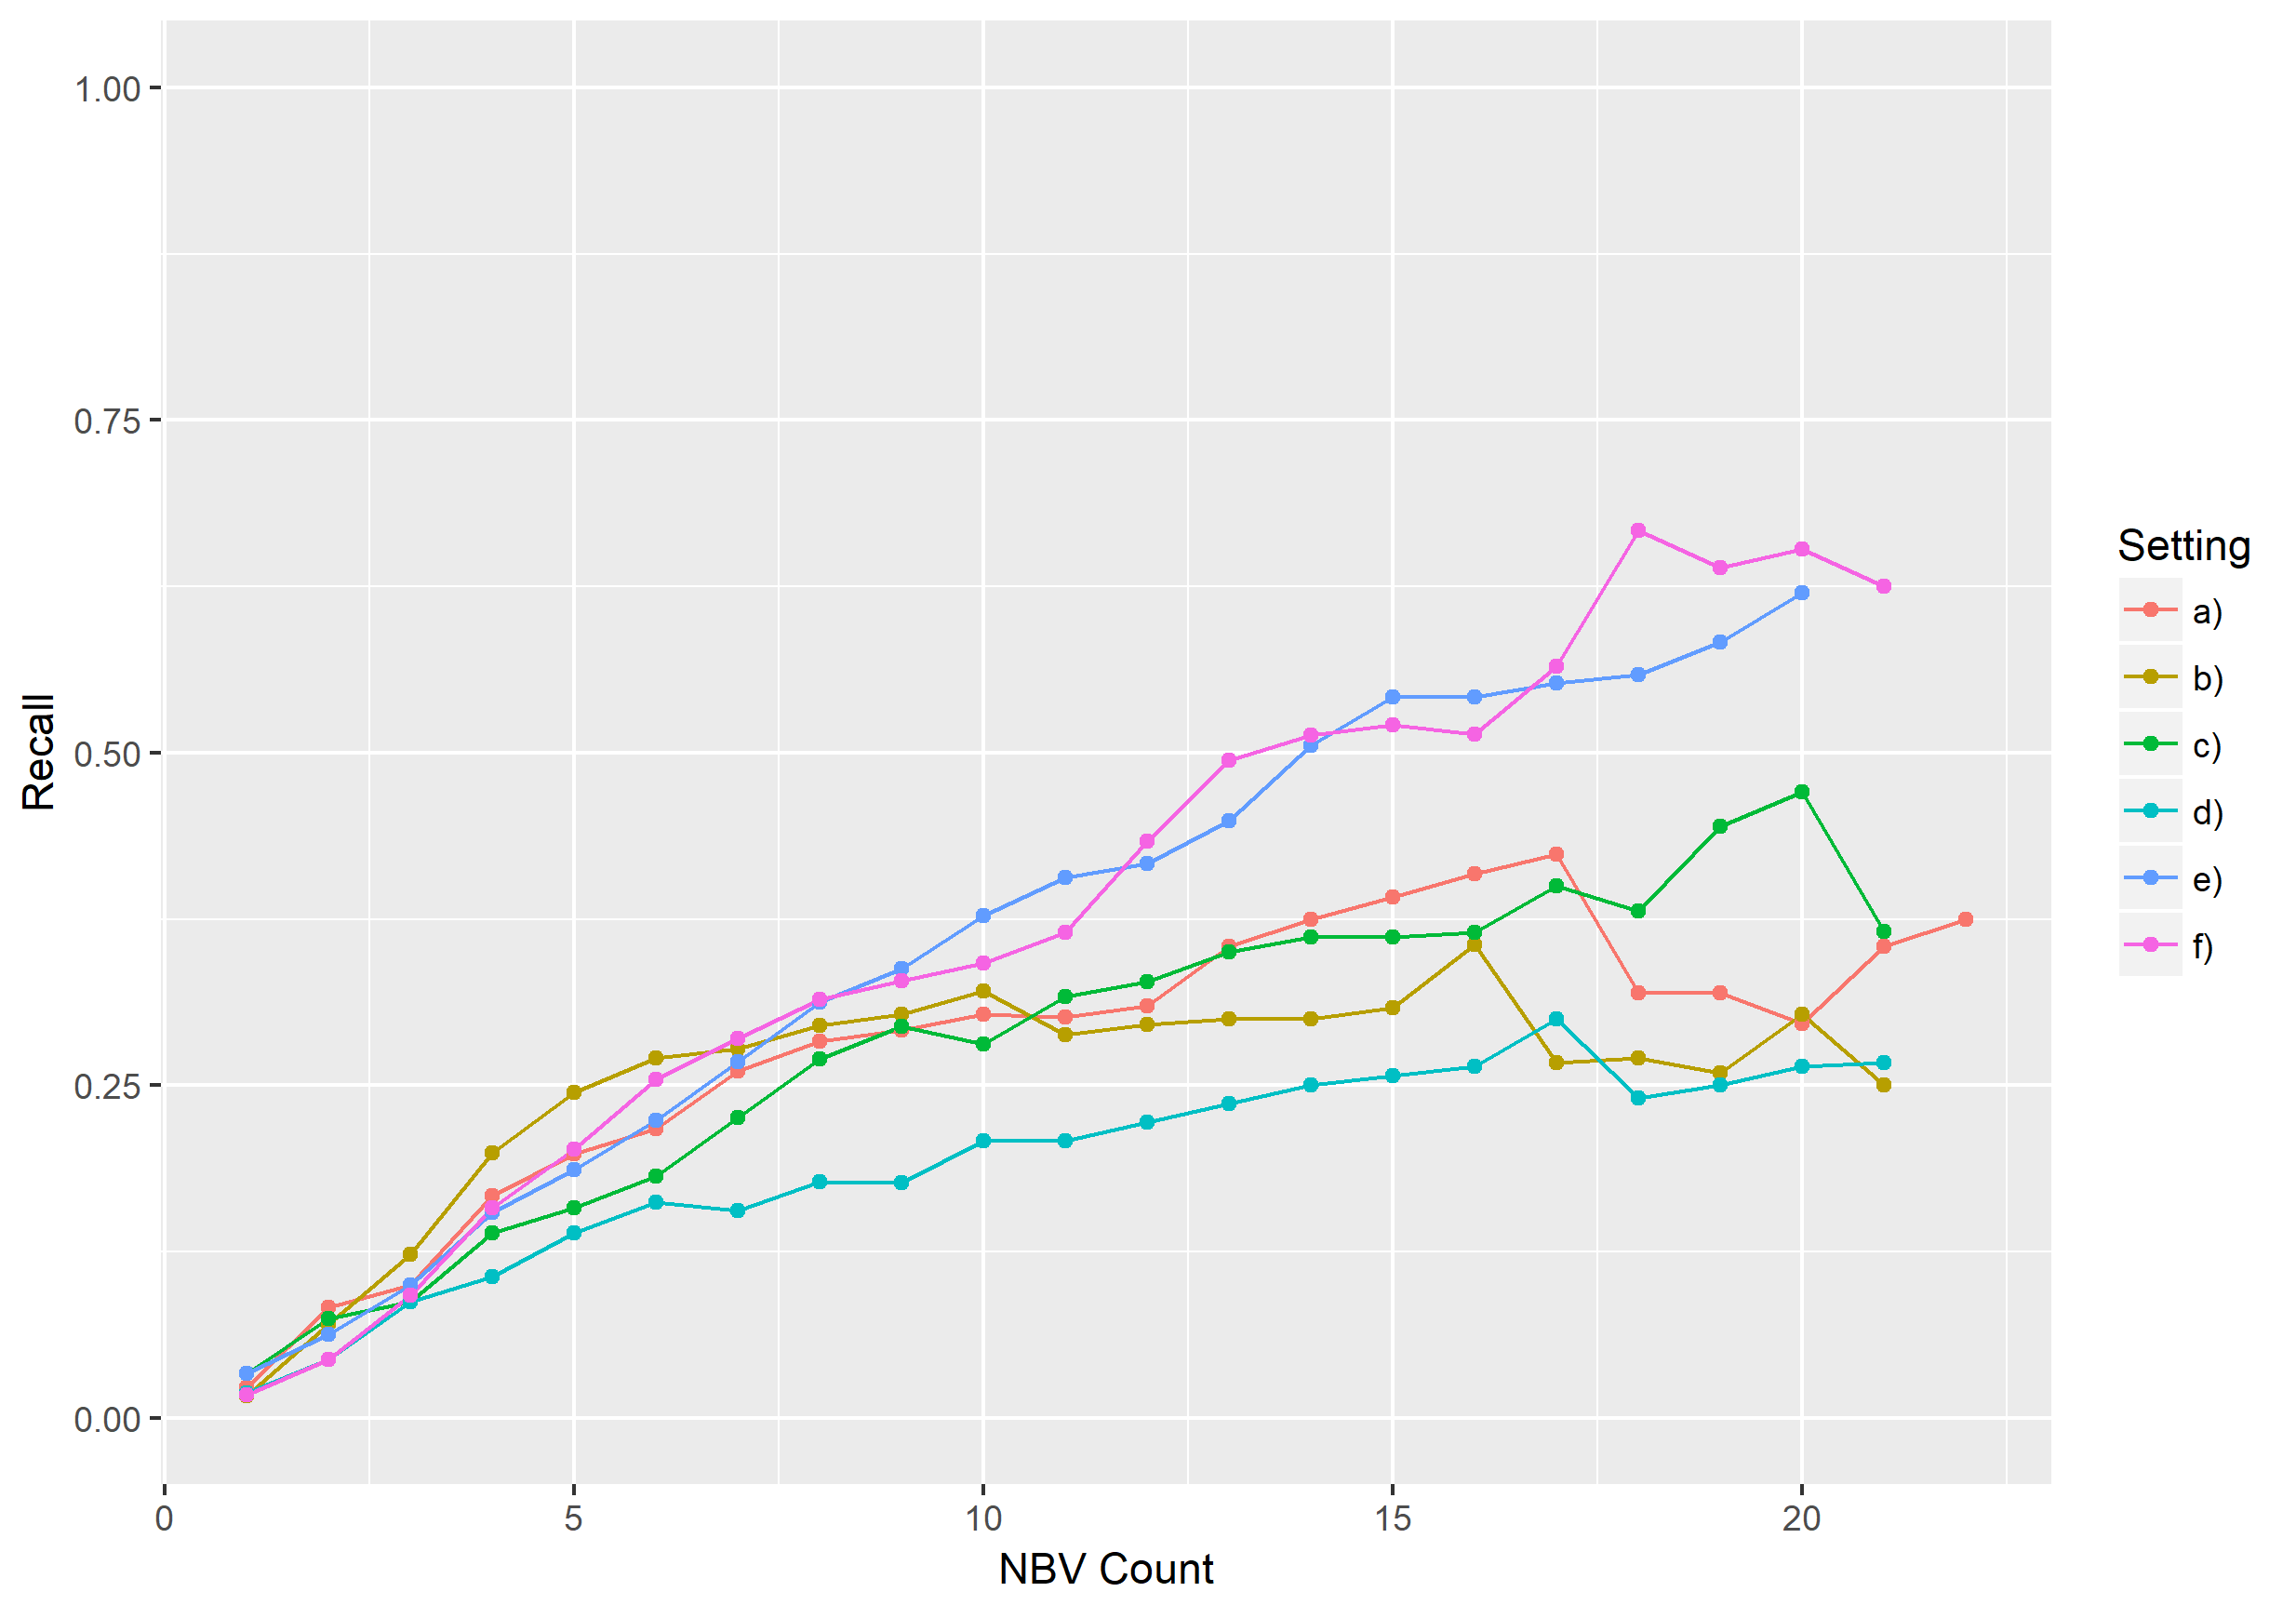
\includegraphics[width=1\textwidth]{src/Plots/setting__recall_vs_nbv_count.png}
		\caption{Recall values for different information gain parameter settings}
		\label{fig:recall_vs_nbv_count_settings}
	\end{center}
\end{figure}

In Figure \ref{fig:recall_vs_nbv_count_settings} different settings for the information gain parameters of our SBE methods are visualized in their effect on the recall. Precision is not strongly affected by the different settings.
The best performing settings are f) and e). In both of these setting information gain is only provided for cells containing obstacles, in e) a bonus is given for unexplored cells in front of obstacles (e) corresponds to \texttt{SBE (obs)}).
Setting a) is using the parameters from \texttt{SBE (obs+cands)} and b) is similar, but information gain through objects candidates is halved. c) is also related to a), but non of the bonuses for unexplored cells in front of obstacles or object candidates are given. These three settings perform similar, but much worse than the obstacle focused settings. This corresponds to the overall worse performing \texttt{SBE(Obs+Cands)} method.
The worst performing setting is d) where information gain is solely provided for cells containing object candidates. This fits to our previous results since this is the only setting that is not considering obstacles for the information gain calculations.

%\begin{figure}[h!]
%	\begin{center}
%		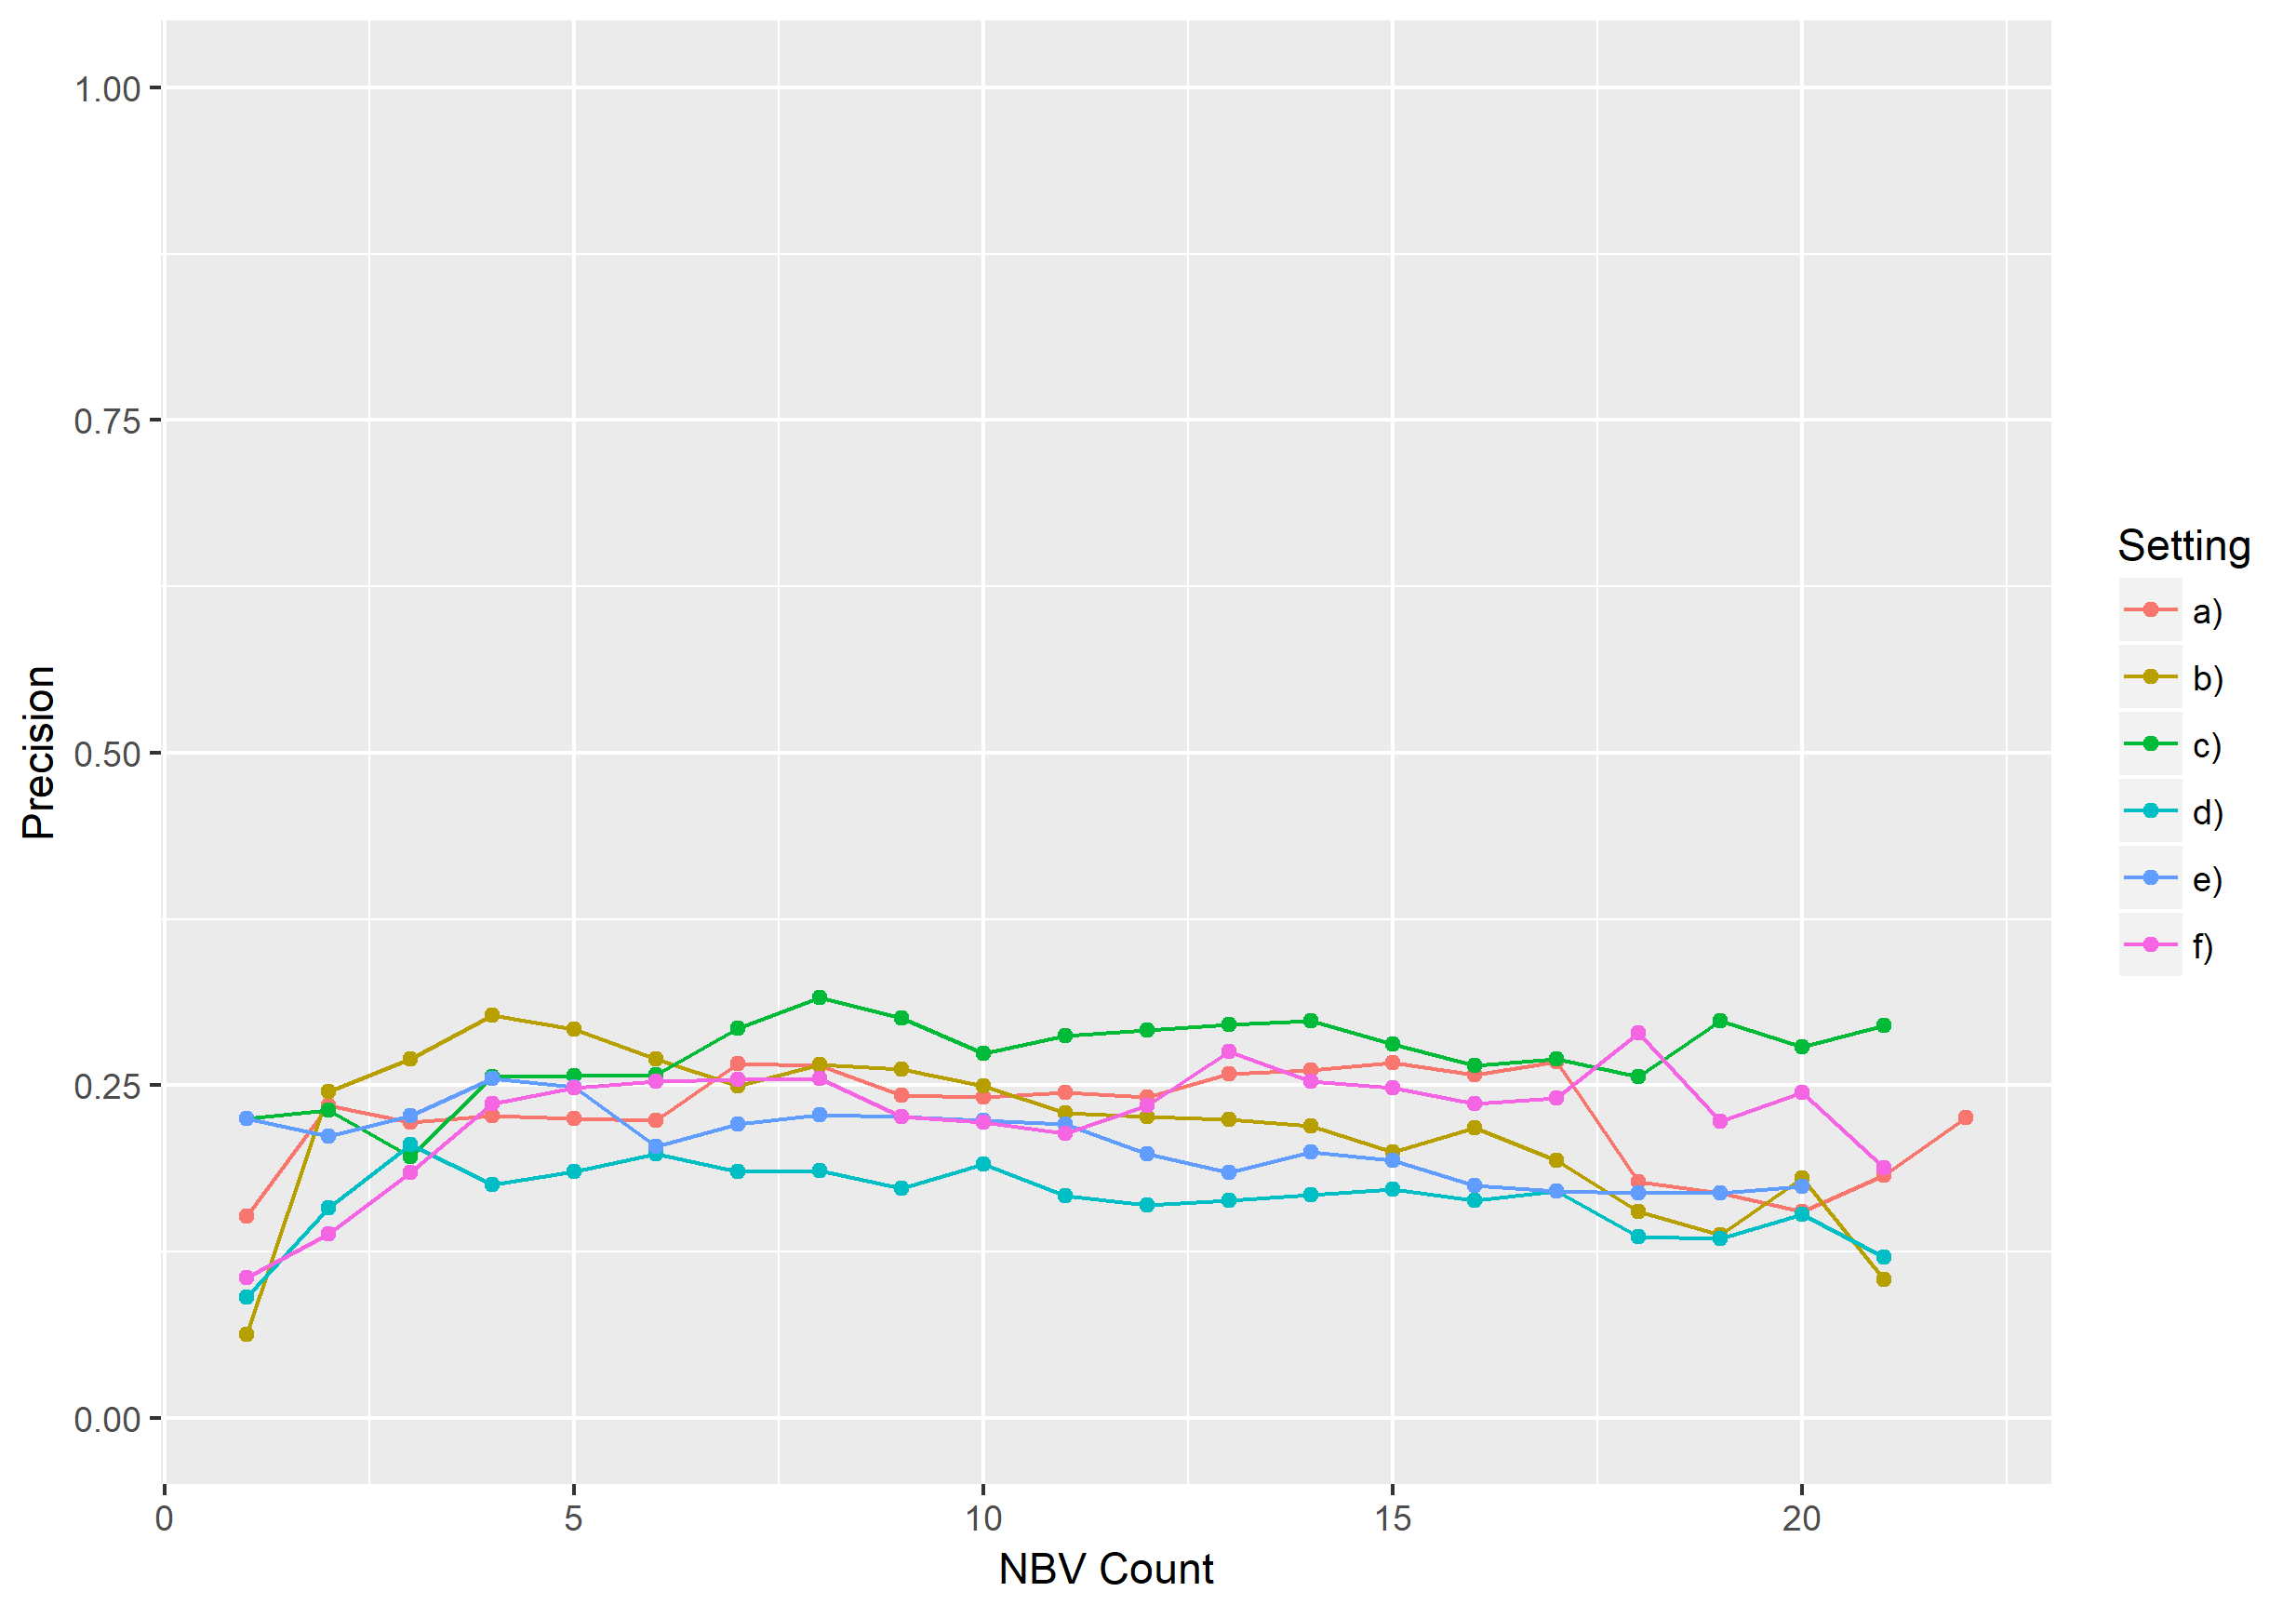
\includegraphics[width=1\textwidth]{src/Plots/setting__precision_vs_nbv_count.png}
%		\caption{Precision values for different information gain parameter settings}
%		\label{fig:precision_vs_nbv_count_settings}
%	\end{center}
%\end{figure}

\begin{figure}[h!]
	\begin{center}
		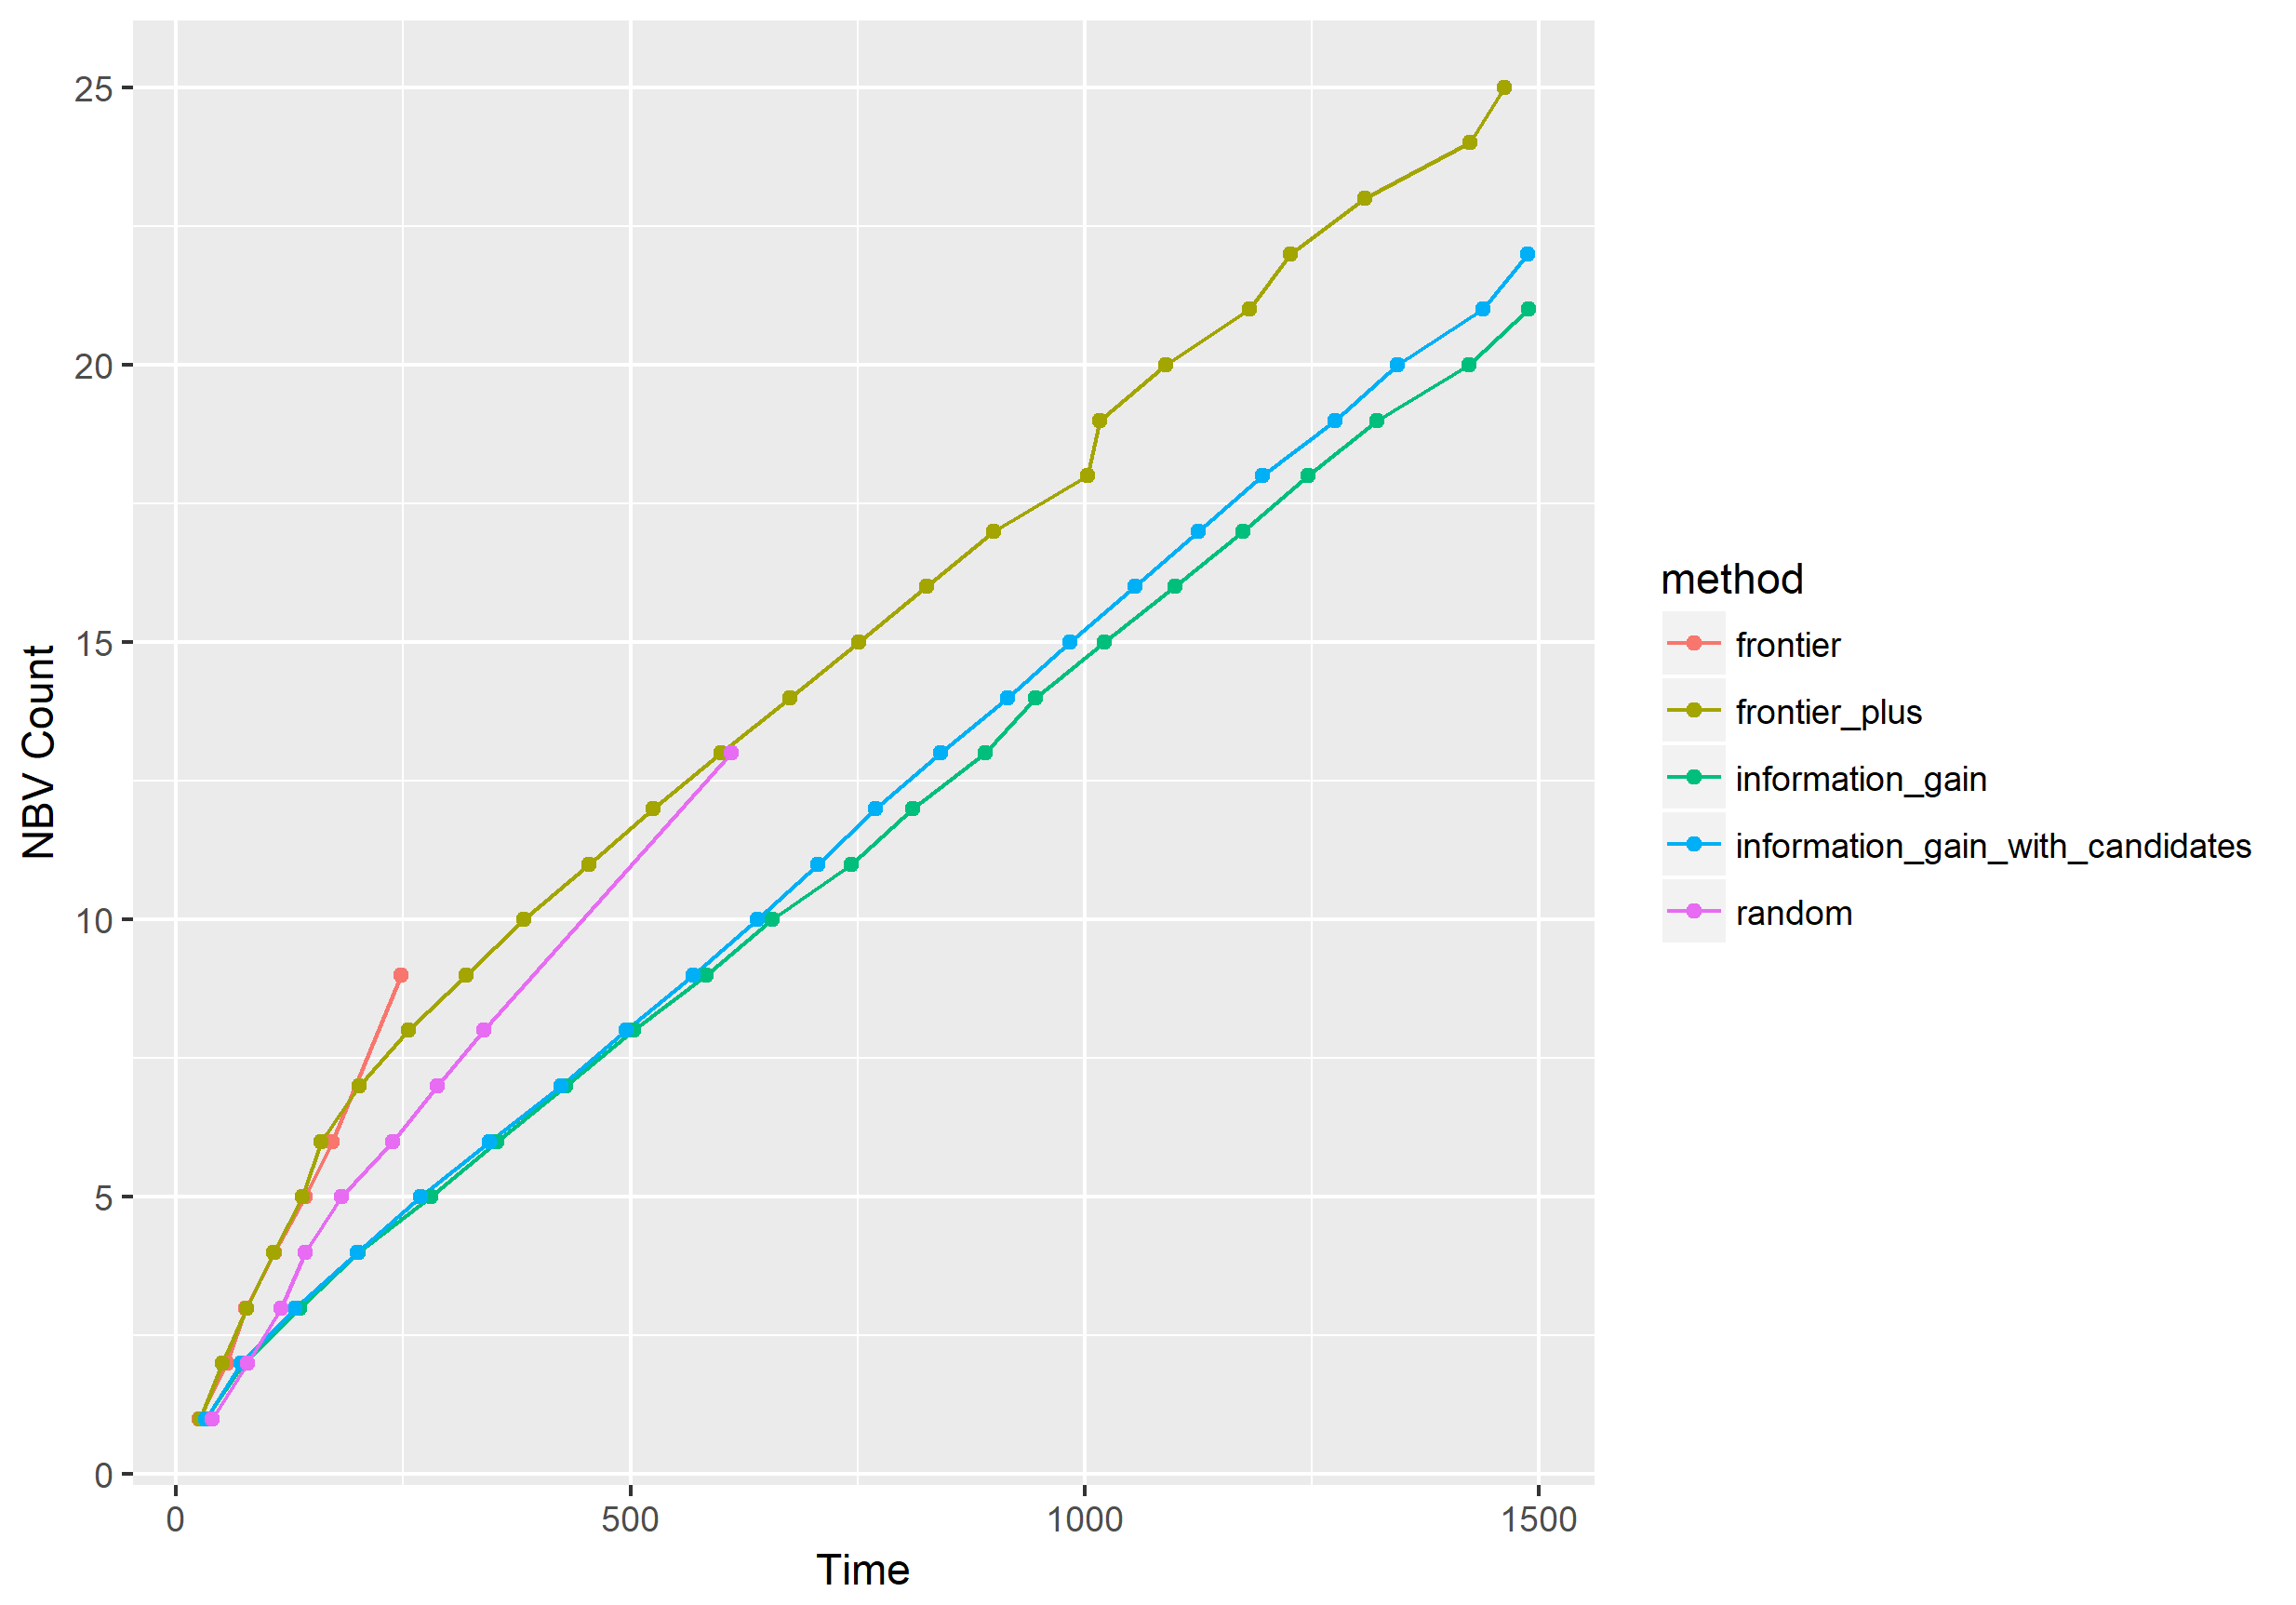
\includegraphics[width=1\textwidth]{src/Plots/nbv_count_vs_time.png}
		\caption{Time used per view taken for all methods}
		\label{fig:nbv_count_vs_time}
	\end{center}
\end{figure}

In Figure \ref{fig:nbv_count_vs_time} the average time required to perform a certain number of views can be seen. 
Interestingly the \texttt{FBE} method is even faster than \texttt{random NBV}, this is because the random views can be far apart from each other, which leads Unsurprisingly, the \texttt{SBE} methods are the slowest solutions, because the computation of sophisticated information gain for many accessible cells is costly. In this graph the \texttt{FBE plus} method can show its advantage against the other \texttt{SBE} methods, because its  benefiting from the fast frontier exploration at the beginning.

\section{Conclusion}
\label{Conclusion}

%!TEX root = ../final_report.tex

%Conclusions, which summarizes the work that was done and the results obtained, and gives suggestions for future work. \textbf{Most importantly}, include a section that contrasts the actual outcome of the project to the plan you submitted: what was planned, what was actually achieved, what were the main reasons for the actual outcome, what you consider you have learned during the project, etc.

\subsection{Summary}

The project successfully achieved its aim of developing a system for autonomous object discovery on a mobile robot in an unknown environment and using it to test NBV algorithms.
As well as the NBV algorithms themselves, modules were developed for object candidate detection in 2D and for projection of the 2D candidates into 3D; these were combined with off-the-shelf solutions for SLAM, navigation and robot control.
The experiments were performed in simulation to allow us to fully control the environment and automate the testing process.
The system was also shown to work on a real robot, however the input which the system received from the real Kinect was too noisy for the SLAM system to cope with, which meant the system could not effectively map and navigate a real world environment for more than a couple of minutes before the navigation module failed.
Among the NBV algorithms which we implemented, all which used information gain outperformed the random algorithm.
The best performing was the \texttt{SBE(Obs)} method, with recall of \num{0.75} and precision of \num{0.25} after \num{25} views.

\subsection{Reflection}
\label{ssec:reflection}

Looking back on the aims from our initial project proposal, we have achieved everything that we intended, with the minor exception that we did not implement the ``table scenario'' in which objects were positioned on a table and the robot moved around the table to its next best viewpoints, but rather skipped straight to the more complex ``scattered objects scenario'', which we initially planned only as an extension goal.
This was done partly because we felt that restricting the next best view poses to a circle around the table constrained the problem too much and would make it hard to meaningfully assess our different NBV algorithms, and partly because the table scenario turned out to be harder to implement: we would have needed everything that we developed for the scattered object scenario, with the added complication of having separate maps for navigation (the floor) and object discovery (the tabletop).
Accordingly, we focussed our efforts on the more challenging and interesting scenario.
We also achieved our goal of implementing and comparing several different NBV algorithms.

Comparing our actual implementation to the plan we laid out in the intermediate report, we see some significant differences where we discovered during the implementation phase that our original plans needed to be adjusted.

\paragraph{Robot battery life} % (fold)
\label{par:robot_battery_life}

We originally conceived of making our NBV calculations and termination conditions dependent on the robot's remaining battery power.
However, given that our maximum experiment duration was \SI{25}{\minute} and the robot's battery life is several hours, we judged this criterion to be largely superfluous.
Also, performing our experiments in simulation meant that we could bypass the issue of battery life altogether.

% paragraph paragraph_name (end)

\paragraph{Exploration methods} % (fold)
\label{par:exploration_methods}

The sampling-based exploration method derived from Surmann et al. \cite{surmann2003autonomous} was significantly revised during the implementation.
The input to Surmann et al.'s system is purely points in continuous space, detected by a laser range finder, which are assumed to lie on object surfaces.
They do not distinguish between free and unknown space.
In our system by contrast, by the time we come to calculate our next best view we already have a discretized occupancy grid which explicitly tells us about unknown, free and occupied space, and we use this extra information in our calculations.

% paragraph exploration_methods (end)

\paragraph{Additional modules} % (fold)
\label{par:additional_modules}

Some unanticipated problems emerged during the implementation phase which required us to implement several extra elements in the system over and above our original plans:

\begin{itemize}
	\item The poor performance of the Gmapping SLAM system made it necessary to implement the cheat mode in order to get any sensible test results.
	\item The ``rays'' resulting from errors in the 3D projection necessitated the implementation of the point cloud clustering algorithm.
	\item The IoR mechanism became necessary when we found in our early tests that the robot would often take several successive views of the same object(s) rather than trying to explore the whole space.
	\item The unexpectedly good performance of the method using frontier-based exploration led us to implement the \texttt{FBE plus} method.
	\item We originally discussed and then discarded the idea of implementing a random NBV method, only to find during the implementation that it would actually be a useful baseline measure.
\end{itemize}

% paragraph additional_modules (end)

Another thing which surprised us during the project was the time and effort required to create a structure within which we could meaningfully evaluate the system, and then to run the evaluation itself.
By using the YCB object set we saved ourselves from having to physically scan objects, but importing the objects into the Gazebo simulation environment was less straightforward than we expected.
For each object, a mesh and a point cloud is provided, and we used the mesh in the simulation environment and the corresponding point cloud as our ground truth.
However, we discovered that the mesh and the point cloud are not in the same coordinate system, so we had to manually specify a transform for each ground truth in order to ensure that it lined up correctly with what was in the environment.
Additionally, measuring volumes and overlaps in the octomap turned out to be less trivial than we initially believed.

The runtime for our tests is also an issue. Because the simulation runs in real time, each run can take up to \SI{25}{\minute}.
Given that we had many different parameters and methods to test, and that we needed to test each scenario as many times as possible in order to limit the effects of random variation, this meant that simply generating results of a sufficient quality took a very long time.
It also restricted our ability to tune the many parameters which our system contains; some parameters, e.g. the \SI{5}{\percent} threshold mentioned in section \ref{sssec:point_cloud_into_octomap}, were taken directly from the literature and we did not have time to thoroughly explore whether we could optimize these values for our system.
Although our anticipation of how long different tasks would take was generally realistic, the evaluation is one phase where we should have planned in significantly more time.

\subsection{Future work}

If we were to start this project again now, the main thing which we would do differently would be to pay more attention to the SLAM problem, because our finished implementation is severely limited by the poor performance of Gmapping's SLAM.
In our tests, Gmapping had a localization error of as much as a meter in simulation and performed even worse in real world tests, due to the point cloud from the real world Kinect (and thus also the simulated laser scan generated from said point cloud) being so much noisier.

We originally chose to use Gmapping because it is lightweight, allowing us to devote more computational resources to object discovery and NBV, and because it is simple to implement and get running.
However, we did not take into account that the localization accuracy of our own object candidates would be strongly dependent on the quality of the robot localization.
Given this realization, it would make more sense to use a SLAM system which is tailor-made for RGB-D input; one such system which is already implemented for ROS is \texttt{rgbdslam\_v2}\footnote{\url{http://wiki.ros.org/rgbdslam}} from Endres et al.\cite{endres2014rgbdslam}.
Switching to a SLAM system which achieves a better localization accuracy would be the most significant single improvement which could be made to our system.

In our intermediate report, we considered several possible extensions to the system:
\begin{itemize}
	\setlength\itemsep{1pt}
	\item using depth information for the computation of object candidates;
	\item using heuristics to estimate the shape of unseen areas of objects;
	\item implementing a POMDP-based NBV algorithm.
\end{itemize}

All three of these extensions remain open.
The point cloud clustering step in our implemented system does implicitly use depth information, but depth information could be more explicitly applied e.g. by including it in the saliency system.

One drawback of using a saliency-based object detection system is that the saliency of a part of an image is always relative to the overall saliency of that particular image.
In other words, in a mostly featureless image, even small features become highly salient.
In our testing environment, the consequence of this is that if the agent takes an image which does not include any objects but only the wall and floor, then a textured area of the wall can become salient enough in comparison to the rest of the image to be detected as an object candidate.

Experimenting with different threshold values for the absolute saliency required for an area to qualify as a candidate did not yield a satisfactory way of avoiding this without also excluding a large number of genuine candidates.
An alternative solution could be to implement some kind of further heuristic which excludes these kind of candidates, such as placing a limit on candidate size or by detecting and excluding large, flat candidates.



\newpage
\bibliographystyle{plain}
\addcontentsline{toc}{section}{Bibliography}% Add to the TOC
\bibliography{bib}

\end{document}
